\documentclass[12pt,a4paper]{article}

% ================= PACKAGES =================
\usepackage[utf8]{inputenc}
\usepackage[T5]{fontenc}
\usepackage[vietnamese]{babel}
\usepackage{amsmath,amssymb,amsfonts}
\usepackage{geometry}
\geometry{left=2.5cm,right=2.0cm,top=2.5cm,bottom=2.5cm}
\usepackage{graphicx}
\usepackage{booktabs}
\usepackage{longtable}
\usepackage{array}
\usepackage{multirow}
\usepackage{float}
\usepackage{caption}
\usepackage{subcaption}
\usepackage{xcolor}
\usepackage{listings}
\usepackage{tikz}
\usetikzlibrary{shapes.geometric, arrows.meta, positioning}
\usepackage{fancyhdr}
\usepackage{hyperref}

\hypersetup{
    colorlinks=true,
    linkcolor=blue!70!black,
    citecolor=blue!70!black,
    urlcolor=blue!70!black,
    pdftitle={Bao Cao Bai Tap Lon Nhap Mon Hoc May - De Tai 13},
}

% ================= CODE LISTING STYLE =================
\definecolor{codebg}{rgb}{0.97,0.97,0.98}
\definecolor{codegreen}{rgb}{0.1,0.5,0.2}
\definecolor{codegray}{rgb}{0.45,0.45,0.45}
\definecolor{codeblue}{rgb}{0.1,0.2,0.7}

\lstdefinestyle{pythonstyle}{
    language=Python,
    backgroundcolor=\color{codebg},
    commentstyle=\color{codegreen}\itshape,
    keywordstyle=\color{codeblue}\bfseries,
    numberstyle=\tiny\color{codegray},
    stringstyle=\color{red!70!black},
    basicstyle=\ttfamily\footnotesize,
    breakatwhitespace=false,
    breaklines=true,
    captionpos=b,
    keepspaces=true,
    numbers=left,
    numbersep=6pt,
    showspaces=false,
    showstringspaces=false,
    showtabs=false,
    tabsize=4,
    frame=single,
    rulecolor=\color{black!25},
    literate={á}{{\'a}}1 {à}{{\`a}}1 {ả}{{\h{a}}}1 {ã}{{\~a}}1 {ạ}{{\d{a}}}1
             {ă}{{\u{a}}}1 {ắ}{{\'{\u{a}}}}1 {ằ}{{\`{\u{a}}}}1 {ẳ}{{\h{\u{a}}}}1 {ẵ}{{\~{\u{a}}}}1 {ặ}{{\d{\u{a}}}}1
             {â}{{\^a}}1 {ấ}{{\'{\^a}}}1 {ầ}{{\`{\^a}}}1 {ẩ}{{\h{\^a}}}1 {ẫ}{{\~{\^a}}}1 {ậ}{{\d{\^a}}}1
             {đ}{{\dj}}1 {Đ}{{\DJ}}1
             {é}{{\'e}}1 {è}{{\`e}}1 {ẻ}{{\h{e}}}1 {ẽ}{{\~e}}1 {ẹ}{{\d{e}}}1
             {ê}{{\^e}}1 {ế}{{\'{\^e}}}1 {ề}{{\`{\^e}}}1 {ể}{{\h{\^e}}}1 {ễ}{{\~{\^e}}}1 {ệ}{{\d{\^e}}}1
             {í}{{\'i}}1 {ì}{{\`i}}1 {ỉ}{{\h{i}}}1 {ĩ}{{\~i}}1 {ị}{{\d{i}}}1
             {ó}{{\'o}}1 {ò}{{\`o}}1 {ỏ}{{\h{o}}}1 {õ}{{\~o}}1 {ọ}{{\d{o}}}1
             {ô}{{\^o}}1 {ố}{{\'{\^o}}}1 {ồ}{{\`{\^o}}}1 {ổ}{{\h{\^o}}}1 {ỗ}{{\~{\^o}}}1 {ộ}{{\d{\^o}}}1
             {ơ}{{\ohorn}}1 {ớ}{{\'{\ohorn}}}1 {ờ}{{\`{\ohorn}}}1 {ở}{{\h{\ohorn}}}1 {ỡ}{{\~{\ohorn}}}1 {ợ}{{\d{\ohorn}}}1
             {ú}{{\'u}}1 {ù}{{\`u}}1 {ủ}{{\h{u}}}1 {ũ}{{\~u}}1 {ụ}{{\d{u}}}1
             {ư}{{\uhorn}}1 {ứ}{{\'{\uhorn}}}1 {ừ}{{\`{\uhorn}}}1 {ử}{{\h{\uhorn}}}1 {ữ}{{\~{\uhorn}}}1 {ự}{{\d{\uhorn}}}1
             {ý}{{\'y}}1 {ỳ}{{\`y}}1 {ỷ}{{\h{y}}}1 {ỹ}{{\~y}}1 {ỵ}{{\d{y}}}1
}
\lstset{style=pythonstyle}

% ================= HEADER / FOOTER =================
\pagestyle{fancy}
\fancyhf{}
\fancyhead[L]{\small Học phần: Nhập môn Học máy (FIT4013)}
\fancyhead[R]{\small Đề tài 13: Dự đoán nhân viên nghỉ việc}
\fancyfoot[C]{\thepage}
\renewcommand{\headrulewidth}{0.4pt}

\begin{document}

% ================= TITLE PAGE =================
\begin{titlepage}
    \centering
    \vspace*{1cm}
    {\Large \textbf{BÁO CÁO BÀI TẬP LỚN}}\\[0.3cm]
    {\Large \textbf{HỌC PHẦN: NHẬP MÔN HỌC MÁY (FIT4013)}}\\[0.3cm]
    {\large Năm học: 2026 -- 2027}\\[1.8cm]

    \rule{\linewidth}{0.6mm}\\[0.5cm]
    {\huge \textbf{ĐỀ TÀI 13}}\\[0.4cm]
    {\LARGE \textbf{DỰ ĐOÁN NHÂN VIÊN CÓ KHẢ NĂNG NGHỈ VIỆC}}\\[0.2cm]
    {\large \textit{(Nhóm đề tài: Dữ liệu dạng bảng -- Tabular Data)}}\\
    \rule{\linewidth}{0.6mm}\\[1.8cm]

    \begin{minipage}{0.42\textwidth}
        \begin{flushleft} \large
            \textbf{Giảng viên hướng dẫn:}\\
            ThS. Lê Thị Thùy Trang\\[0.3cm]
            \textbf{Nhóm thực hiện:} Nhóm 7
        \end{flushleft}
    \end{minipage}
    \begin{minipage}{0.54\textwidth}
        \begin{flushright} \large
            \textbf{Danh sách thành viên (Nhóm 7):}\\
            1. Nguyễn Văn An -- MSSV: 1871020003\\
            2. Nguyễn Việt Anh -- MSSV: 1871020047\\
            3. Đào Thị Tươi -- MSSV: 1871020639\\
            4. Lê Đình Huy -- MSSV: 1871020307
        \end{flushright}
    \end{minipage}\\[2.5cm]

    \vfill
    {\large Tháng 11 năm 2026}
\end{titlepage}

% ================= ABSTRACT & TOC =================
\begin{abstract}
Báo cáo này trình bày quy trình nghiên cứu, thiết kế và thực nghiệm hoàn chỉnh cho bài toán \textbf{Dự đoán nhân viên có khả năng nghỉ việc (Employee Attrition Prediction)} thuộc nhóm đề tài Dữ liệu dạng bảng (Đề tài 13). Trên bộ dữ liệu tiêu chuẩn IBM HR Analytics gồm $1{,}470$ hồ sơ nhân sự với $35$ thuộc tính, nhóm thực hiện khám phá dữ liệu chuyên sâu (EDA), phát hiện hiện tượng mất cân bằng lớp nghiêm trọng ($83.88\%$ ở lại so với $16.12\%$ nghỉ việc), sự tồn tại của các cột hằng số, cột định danh cũng như hiện tượng đa cộng tuyến giữa các đặc trưng thâm niên và thu nhập. Từ đó, nhóm xây dựng và đối sánh hai luồng chuẩn bị dữ liệu độc lập: \textbf{Luồng A (Pipeline cơ bản)} và \textbf{Luồng B (Pipeline cải tiến)} tích hợp 7 đặc trưng nghiệp vụ nhân sự mới, biến đổi logarit $\log(1+x)$, chuẩn hóa \texttt{RobustScaler} và chọn lọc đặc trưng ANOVA F-test (\texttt{SelectKBest}). Ba thuật toán cốt lõi trong học phần gồm \textbf{K-Nearest Neighbors (K-NN)}, \textbf{Gaussian Naive Bayes} và \textbf{Cây quyết định (Decision Tree)} cùng mô hình mở rộng \textbf{Random Forest} được huấn luyện và tinh chỉnh siêu tham số thông qua kiểm định chéo phân tầng 5-fold (\texttt{StratifiedKFold}). Thực nghiệm trên tập kiểm thử độc lập cho thấy Luồng B giúp nâng cao rõ rệt hiệu quả phát hiện nhân viên nghỉ việc: \texttt{Gaussian Naive Bayes} đạt $F_1 = 0.4821$, $\text{ROC-AUC} = 0.7507$ (tăng từ $F_1 = 0.3687$ ở cấu hình mặc định Luồng A), trong khi \texttt{Decision Tree} tối ưu đạt độ nhạy $\text{Recall} = 68.09\%$ (phát hiện đúng 32/47 nhân viên nghỉ việc). Báo cáo đồng thời phân tích chi tiết các ca dự đoán sai (\textit{False Negatives} và \textit{False Positives}) để đưa ra khuyến nghị quản trị nhân sự thực tiễn.
\end{abstract}

\tableofcontents
\newpage

% =====================================================================
% CHƯƠNG 1: ĐẶT VẤN ĐỀ VÀ PHÂN TÍCH YÊU CẦU
% =====================================================================
\section{Đặt vấn đề và phân tích yêu cầu}

\subsection{Bối cảnh và mục tiêu của bài toán}
Trong quản trị nguồn nhân lực hiện đại, tình trạng nhân viên tự nguyện rời bỏ tổ chức (\textit{Employee Attrition / Turnover}) gây ra tổn thất lớn về chi phí tuyển dụng, chi phí đào tạo lại, gián đoạn tiến độ dự án và chảy máu chất xám. Nếu bộ phận Nhân sự (HR) chỉ nhận biết khi nhân viên đã nộp đơn xin thôi việc thì mọi biện pháp giữ chân đều đã muộn. Do đó, việc ứng dụng Học máy (\textit{Machine Learning}) để dự đoán sớm khả năng nghỉ việc của từng nhân viên dựa trên hồ sơ nhân khẩu học, môi trường làm việc, chế độ đãi ngộ và lộ trình thăng tiến mang ý nghĩa thực tiễn rất cao.

\textbf{Định nghĩa bài toán dưới góc độ Học máy:}
\begin{itemize}
    \item \textbf{Loại bài toán:} Phân loại nhị phân có giám sát (\textit{Supervised Binary Classification}) trên dữ liệu dạng bảng (\textit{Tabular Data}).
    \item \textbf{Đầu vào ($\mathbf{x} \in \mathbb{R}^d$):} Vector đặc trưng mô tả thông tin của một nhân viên (tuổi, thu nhập hàng tháng, làm thêm giờ, tần suất đi công tác, mức độ hài lòng, số năm làm việc, v.v.).
    \item \textbf{Đầu ra ($y \in \{0, 1\}$):} Nhãn mục tiêu \texttt{Attrition}, trong đó:
    \begin{itemize}
        \item $y = 1$ (\texttt{Yes}): Nhân viên có khả năng nghỉ việc (lớp dương -- \textit{Positive class}, đối tượng trọng tâm cần phát hiện).
        \item $y = 0$ (\texttt{No}): Nhân viên tiếp tục gắn bó với công ty (lớp âm -- \textit{Negative class}).
    \end{itemize}
    \item \textbf{Giả định và giới hạn:} Dữ liệu phản ánh trạng thái tĩnh (\textit{cross-sectional snapshot}) của nhân viên tại thời điểm khảo sát, không bao gồm biến động kinh tế vĩ mô bên ngoài hoặc dữ liệu chuỗi thời gian theo từng tháng.
\end{itemize}

\subsection{Khám phá và phân tích dữ liệu (EDA)}

\subsubsection{Nguồn dữ liệu, kích thước và cấu trúc tổng quát}
Bộ dữ liệu sử dụng trong đề tài là \textbf{IBM HR Analytics Employee Attrition \& Performance} (\texttt{WA\_Fn-UseC\_-HR-Employee-Attrition.csv}) do giảng viên chỉ định cho Đề tài 13. Qua kiểm tra bằng mã nguồn Python:
\begin{itemize}
    \item \textbf{Kích thước:} $1{,}470$ bản ghi (tương ứng $1{,}470$ nhân viên) $\times$ $35$ cột ($34$ cột đặc trưng đầu vào và $1$ cột mục tiêu \texttt{Attrition}).
    \item \textbf{Kiểu dữ liệu:} Gồm $26$ cột kiểu số nguyên (\texttt{int64}) và $9$ cột kiểu chuỗi ký tự/phân loại (\texttt{object}).
    \item \textbf{Dữ liệu thiếu (\textit{Missing values}) và trùng lặp (\textit{Duplicates}):} Toàn bộ $35$ cột đều có đúng $1{,}470$ giá trị hợp lệ ($0$ giá trị khuyết) và $0$ bản ghi trùng lặp.
    \item \textbf{Phát hiện các cột dư thừa / định danh:}
    \begin{enumerate}
        \item Ba cột hằng số có phương sai bằng $0$ (chỉ nhận duy nhất 1 giá trị trên toàn bộ $1{,}470$ dòng): \texttt{EmployeeCount} ($= 1$), \texttt{Over18} ($= \text{`Y'}$), và \texttt{StandardHours} ($= 80$).
        \item Một cột định danh duy nhất: \texttt{EmployeeNumber} (nhận $1{,}470$ mã số khác nhau), không mang thông tin tổng quát hóa và có thể gây học vẹt nếu đưa vào mô hình.
    \end{enumerate}
\end{itemize}

Bảng \ref{tab:feature_groups} tóm tắt phân nhóm ý nghĩa của các thuộc tính trong bộ dữ liệu.

\begin{table}[H]
\centering
\caption{Phân nhóm các thuộc tính trong bộ dữ liệu IBM HR Analytics}
\label{tab:feature_groups}
\footnotesize
\begin{tabular}{p{3.5cm} p{7.2cm} p{4.2cm}}
\toprule
\textbf{Nhóm thuộc tính} & \textbf{Các cột tiêu biểu} & \textbf{Đặc điểm & Kiểu dữ liệu} \\
\midrule
Biến mục tiêu & \texttt{Attrition} (\texttt{Yes} / \texttt{No}) & Phân loại nhị phân (16.1\% Yes) \\
Định danh \& Hằng số & \texttt{EmployeeNumber}, \texttt{EmployeeCount}, \texttt{Over18}, \texttt{StandardHours} & Không mang thông tin dự đoán (Cần loại bỏ) \\
Nhân khẩu học & \texttt{Age}, \texttt{Gender}, \texttt{MaritalStatus}, \texttt{Education}, \texttt{EducationField}, \texttt{DistanceFromHome} & Kết hợp số liên tục, thứ bậc (1--5) và định danh \\
Công việc \& Tổ chức & \texttt{Department}, \texttt{JobRole}, \texttt{JobLevel}, \texttt{BusinessTravel}, \texttt{OverTime} & Phân loại định danh và thứ bậc công việc \\
Lương thưởng \& Đãi ngộ & \texttt{MonthlyIncome}, \texttt{PercentSalaryHike}, \texttt{StockOptionLevel}, \texttt{DailyRate}, \texttt{HourlyRate}, \texttt{MonthlyRate} & Số liên tục và mức quyền chọn cổ phiếu (0--3) \\
Thái độ \& Hài lòng & \texttt{JobSatisfaction}, \texttt{EnvironmentSatisfaction}, \texttt{RelationshipSatisfaction}, \texttt{WorkLifeBalance}, \texttt{JobInvolvement} & Biến thứ bậc thang điểm Likert từ 1 (Thấp) đến 4 (Rất cao) \\
Thâm niên \& Lộ trình & \texttt{TotalWorkingYears}, \texttt{YearsAtCompany}, \texttt{YearsInCurrentRole}, \texttt{YearsSinceLastPromotion}, \texttt{YearsWithCurrManager}, \texttt{NumCompaniesWorked} & Số nguyên không âm, phân phối lệch phải mạnh \\
\bottomrule
\end{tabular}
\end{table}

\subsubsection{Phân tích phân phối biến mục tiêu (\texttt{Attrition})}
Hình \ref{fig:target_dist} minh họa phân phối của biến mục tiêu \texttt{Attrition}. Trong tổng số $1{,}470$ nhân viên, có $1{,}233$ nhân viên ở lại (\texttt{No}, chiếm $\mathbf{83.88\%}$) và chỉ có $237$ nhân viên nghỉ việc (\texttt{Yes}, chiếm $\mathbf{16.12\%}$). Tỷ lệ mất cân bằng giữa hai lớp là khoảng $5.20 : 1$.

\begin{figure}[H]
    \centering
    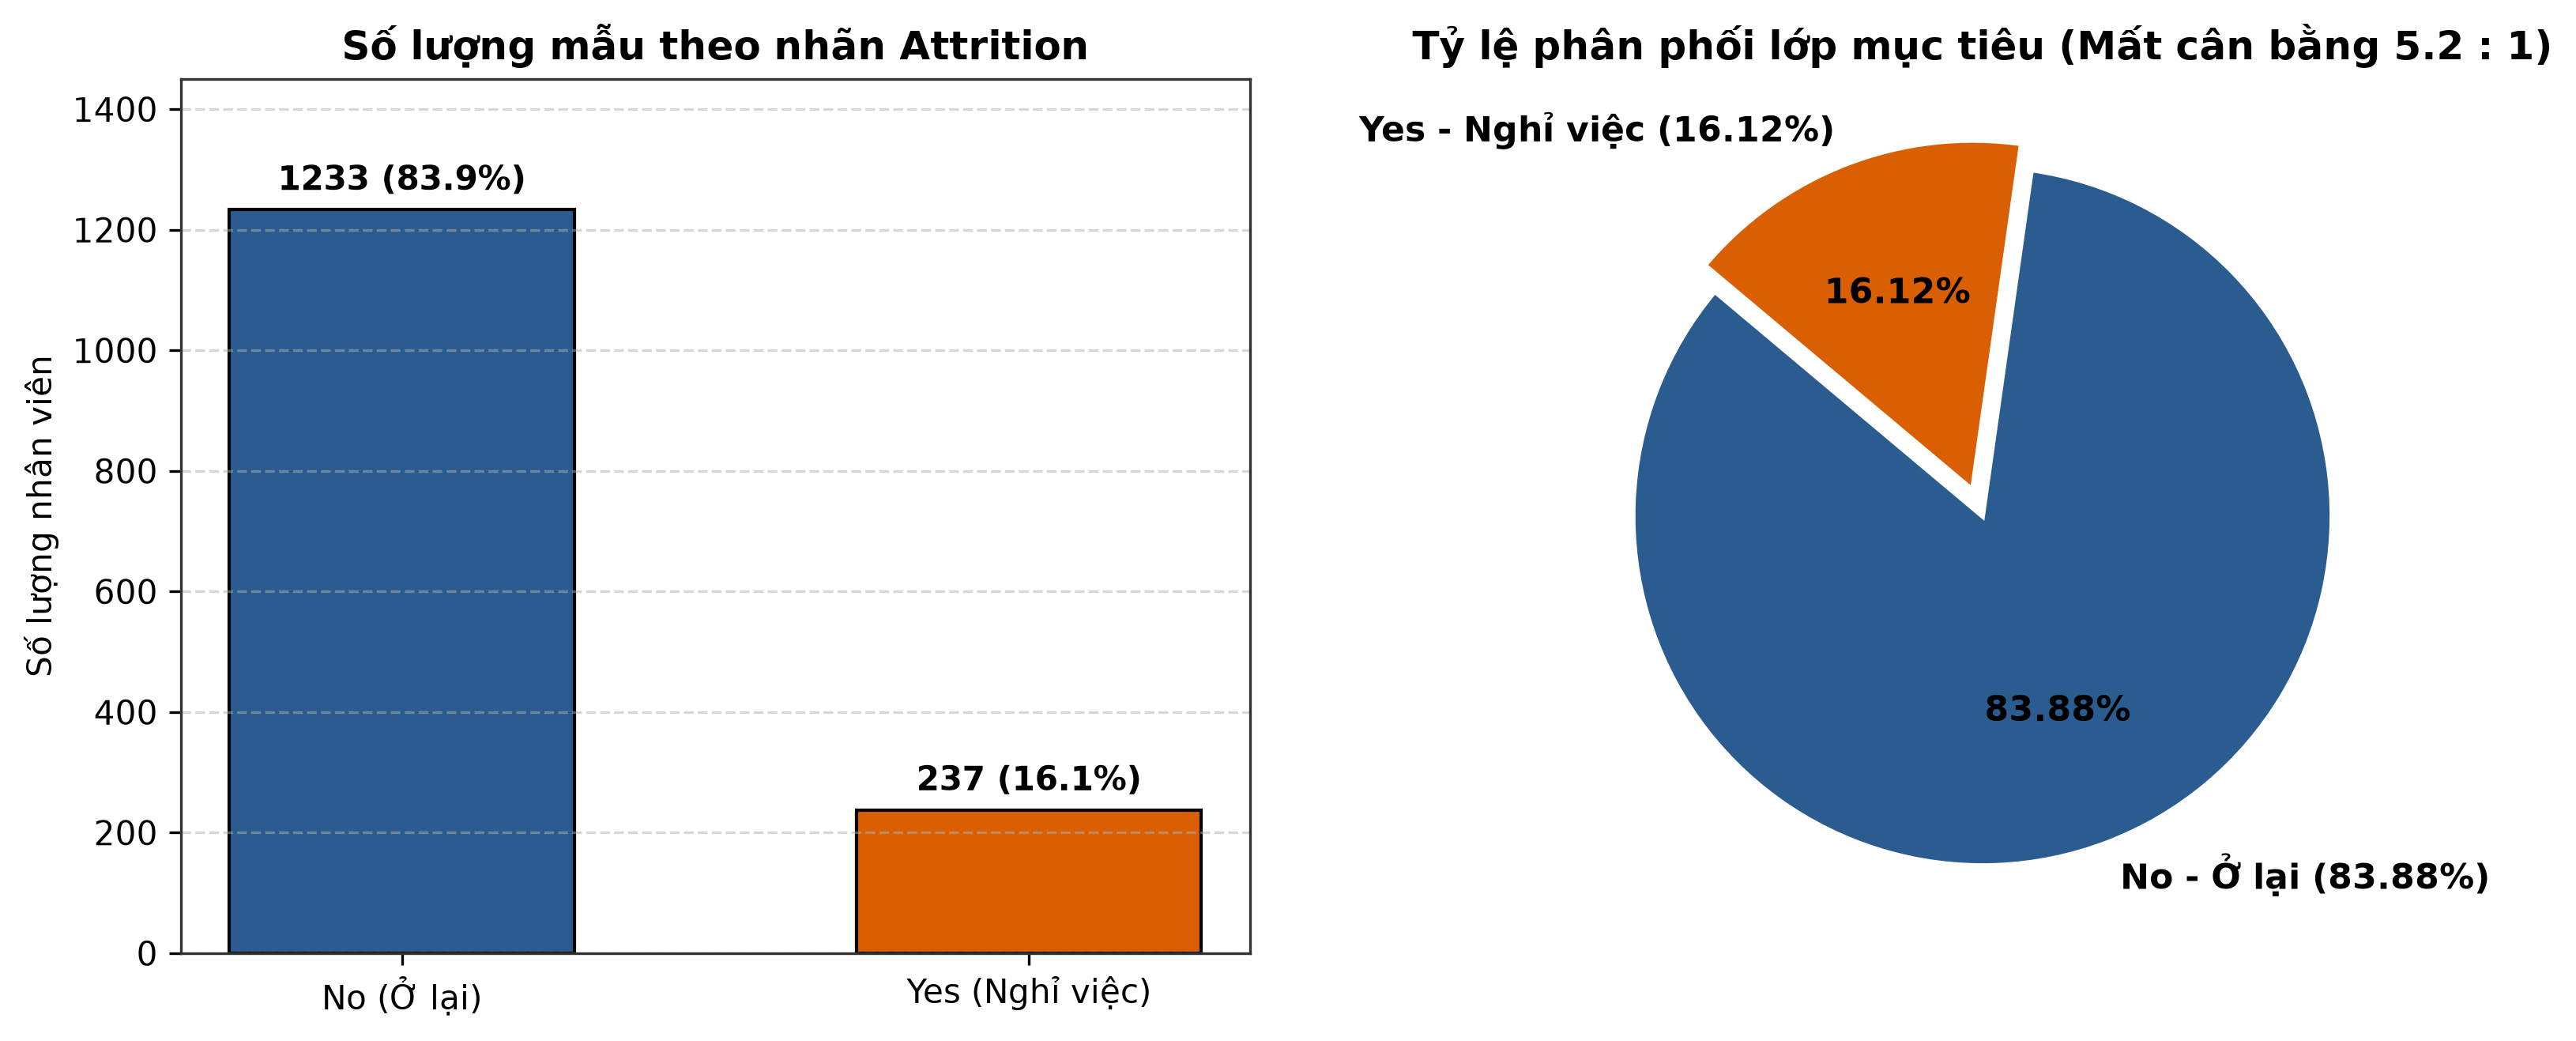
\includegraphics[width=0.92\textwidth]{figures/fig1_target_distribution.png}
    \caption{Phân phối số lượng và tỷ lệ phần trăm của biến mục tiêu \texttt{Attrition}.}
    \label{fig:target_dist}
\end{figure}

Hiện tượng mất cân bằng lớp này đặt ra hai yêu cầu kỹ thuật bắt buộc: (1) Khi chia dữ liệu huấn luyện/kiểm thử phải dùng phương pháp phân tầng (\texttt{stratify=y}); (2) Không được đánh giá mô hình chỉ dựa trên \texttt{Accuracy}, mà phải ưu tiên \texttt{Precision}, \texttt{Recall}, \texttt{F1-score} của lớp dương (\texttt{Yes}) và diện tích dưới đường cong \texttt{ROC-AUC}.

\subsubsection{Phân tích đặc trưng số, ngoại lệ và đặc trưng phân loại}
Bảng \ref{tab:numeric_stats} trình bày thống kê mô tả, hệ số bất đối xứng (\textit{Skewness}) và số lượng điểm ngoại lệ xác định theo quy tắc khoảng tứ phân vị ($\text{IQR} = Q_3 - Q_1$, ngoại lệ khi $x < Q_1 - 1.5\text{IQR}$ hoặc $x > Q_3 + 1.5\text{IQR}$) của các đặc trưng số liên tục.

\begin{table}[H]
\centering
\caption{Thống kê mô tả, độ lệch (\textit{Skewness}) và số lượng ngoại lệ IQR của các đặc trưng số.}
\label{tab:numeric_stats}
\footnotesize
\begin{tabular}{l r r r r r r r r r}
\toprule
\textbf{Đặc trưng} & \textbf{Mean} & \textbf{Std} & \textbf{Min} & \textbf{25\%} & \textbf{50\%} & \textbf{75\%} & \textbf{Max} & \textbf{Skew} & \textbf{Outliers (\%)} \\
\midrule
\texttt{Age}                     & 36.92 & 9.14    & 18   & 30.0  & 36.0  & 43.0  & 60    & 0.41  & 0 (0.00\%) \\
\texttt{MonthlyIncome}           & 6502.93 & 4707.96 & 1009 & 2911.0 & 4919.0 & 8379.0 & 19999 & \textbf{1.37}  & \textbf{114 (7.76\%)} \\
\texttt{DistanceFromHome}        & 9.19  & 8.11    & 1    & 2.0   & 7.0   & 14.0  & 29    & 0.96  & 0 (0.00\%) \\
\texttt{TotalWorkingYears}       & 11.28 & 7.78    & 0    & 6.0   & 10.0  & 15.0  & 40    & \textbf{1.12}  & \textbf{63 (4.29\%)} \\
\texttt{YearsAtCompany}          & 7.01  & 6.13    & 0    & 3.0   & 5.0   & 9.0   & 40    & \textbf{1.76}  & \textbf{104 (7.07\%)} \\
\texttt{YearsInCurrentRole}      & 4.23  & 3.62    & 0    & 2.0   & 3.0   & 7.0   & 18    & 0.92  & 21 (1.43\%) \\
\texttt{YearsSinceLastPromotion} & 2.19  & 3.22    & 0    & 0.0   & 1.0   & 3.0   & 15    & \textbf{1.98}  & \textbf{107 (7.28\%)} \\
\texttt{YearsWithCurrManager}    & 4.12  & 3.57    & 0    & 2.0   & 3.0   & 7.0   & 17    & 0.83  & 14 (0.95\%) \\
\texttt{NumCompaniesWorked}      & 2.69  & 2.50    & 0    & 1.0   & 2.0   & 4.0   & 9     & 1.03  & 52 (3.54\%) \\
\texttt{PercentSalaryHike}       & 15.21 & 3.66    & 11   & 12.0  & 14.0  & 18.0  & 25    & 0.82  & 0 (0.00\%) \\
\texttt{TrainingTimesLastYear}   & 2.80  & 1.29    & 0    & 2.0   & 3.0   & 3.0   & 6     & 0.55  & 238 (16.19\%) \\
\bottomrule
\end{tabular}
\end{table}

Hình \ref{fig:num_hist} và Hình \ref{fig:num_dist} lần lượt thể hiện biểu đồ phân phối tần suất (\textit{Histogram + KDE}) và biểu đồ hộp (\textit{Boxplot}) của 6 đặc trưng số tiêu biểu phân tách theo nhãn \texttt{Attrition}. Quan sát biểu đồ và bảng thống kê mô tả cho thấy:
\begin{itemize}
    \item Nhân viên nghỉ việc (\texttt{Yes}) có độ tuổi trung vị thấp hơn ($32$ tuổi so với $36$ tuổi ở nhóm \texttt{No}) và mức thu nhập hàng tháng (\texttt{MonthlyIncome}) thấp hơn rõ rệt (trung vị $\$3{,}202$ so với $\$5{,}204$ của nhóm ở lại).
    \item Khoảng cách từ nhà đến công ty (\texttt{DistanceFromHome}) của nhóm nghỉ việc cao hơn nhóm ở lại.
    \item Các biến \texttt{MonthlyIncome} ($\text{Skew}=1.37$, $114$ ngoại lệ), \texttt{TotalWorkingYears} ($\text{Skew}=1.12$, $63$ ngoại lệ), \texttt{YearsAtCompany} ($\text{Skew}=1.76$, $104$ ngoại lệ) và \texttt{YearsSinceLastPromotion} ($\text{Skew}=1.98$, $107$ ngoại lệ) bị \textbf{lệch phải mạnh (\textit{right-skewed})} và xuất hiện nhiều điểm ngoại lệ ở vùng giá trị lớn. Điều này sẽ ảnh hưởng trực tiếp tới thuật toán tính khoảng cách như K-NN và giả định phân phối chuẩn của Gaussian Naive Bayes nếu chỉ chuẩn hóa tuyến tính thông thường.
\end{itemize}

\begin{figure}[H]
    \centering
    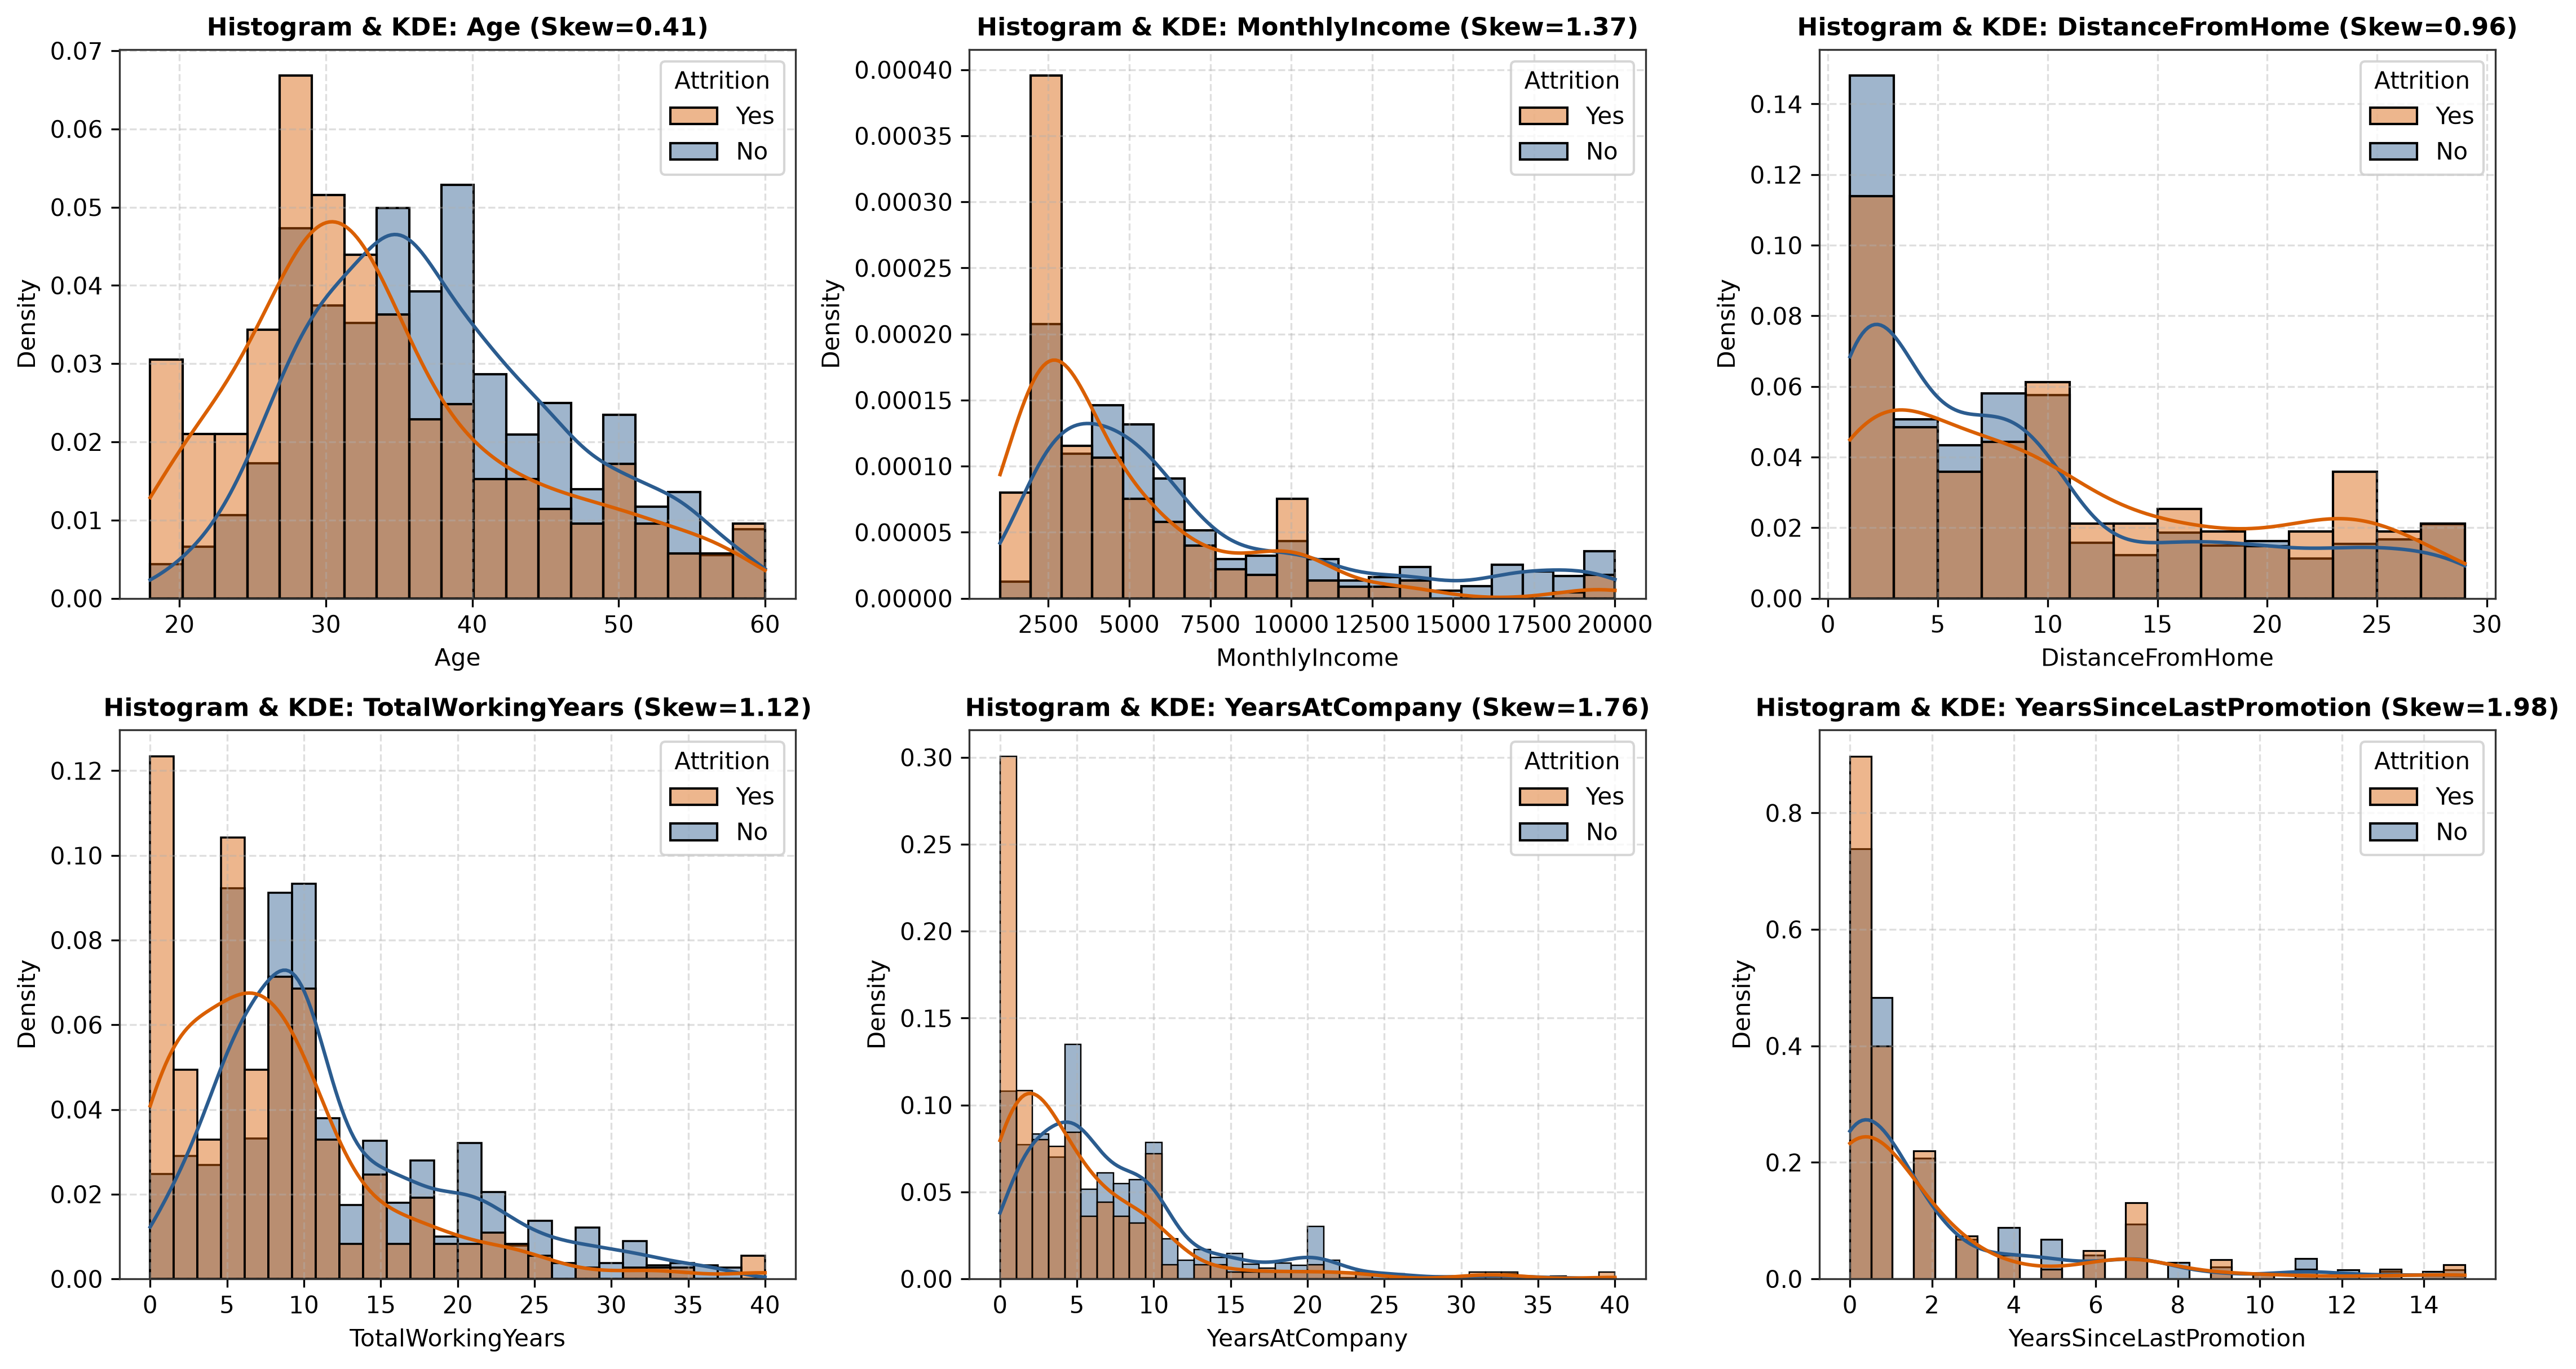
\includegraphics[width=0.98\textwidth]{figures/fig10_numeric_histograms.png}
    \caption{Biểu đồ Histogram và ước lượng mật độ hạt nhân (KDE) của 6 đặc trưng số theo \texttt{Attrition}.}
    \label{fig:num_hist}
\end{figure}

\begin{figure}[H]
    \centering
    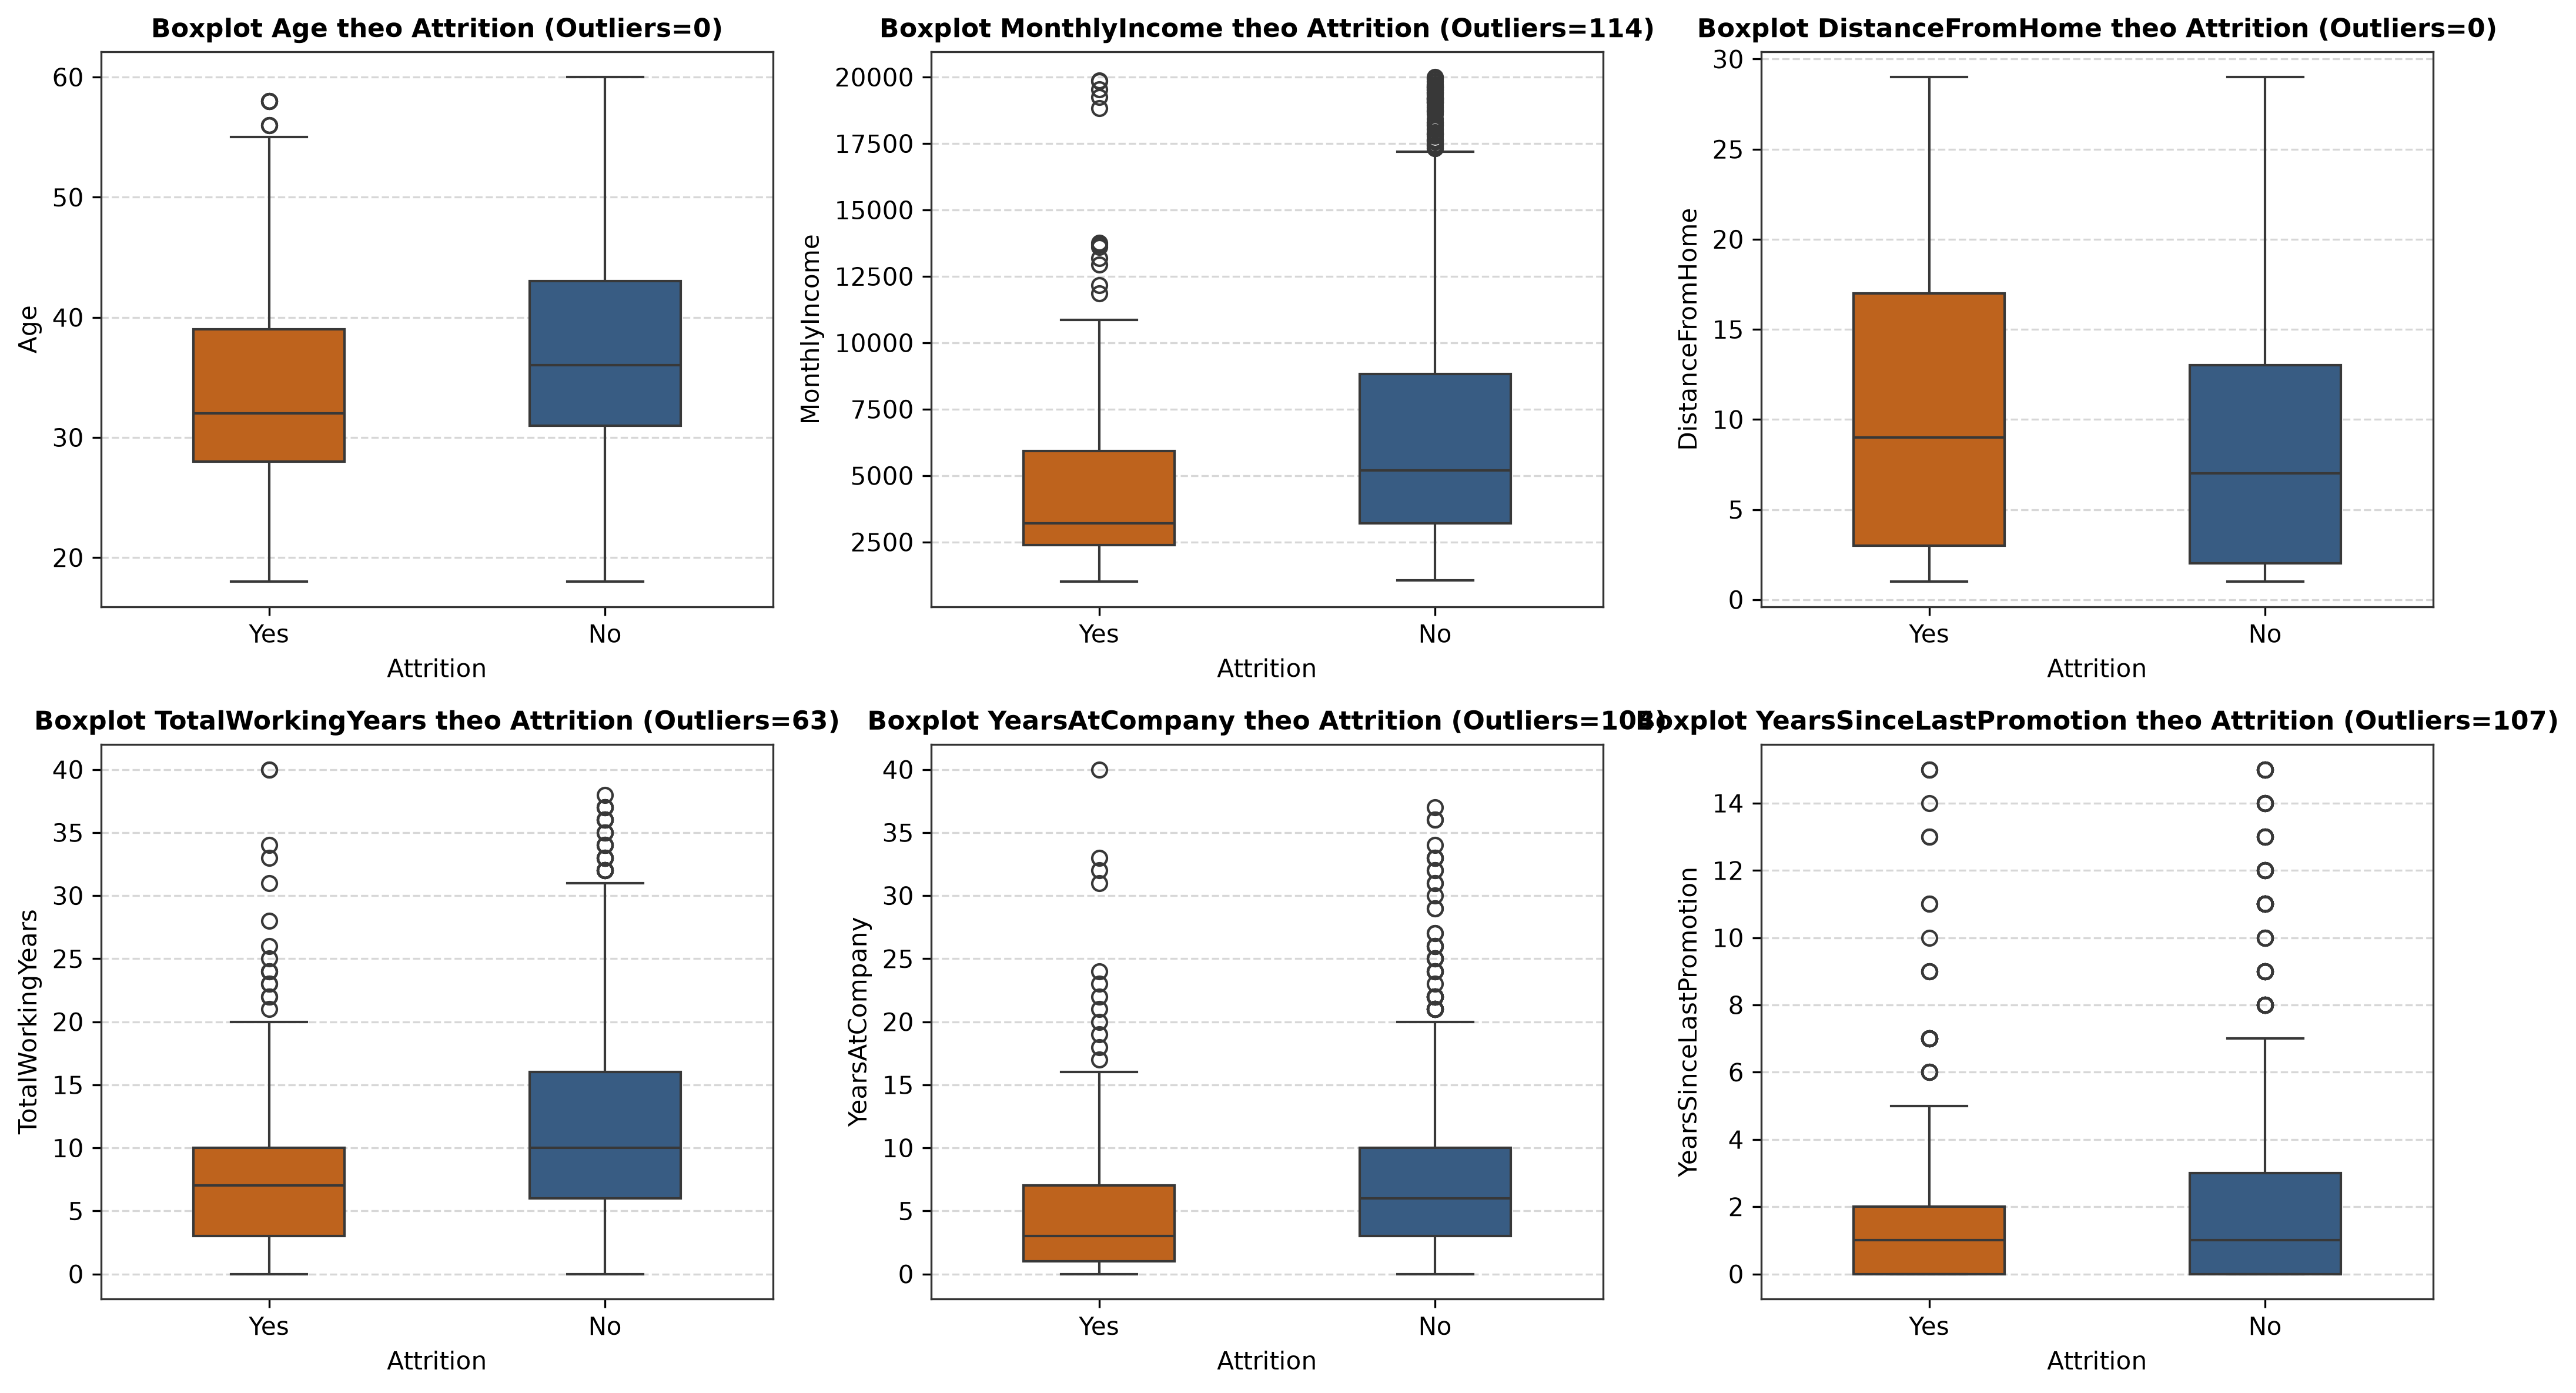
\includegraphics[width=0.98\textwidth]{figures/fig2_numeric_distributions.png}
    \caption{Biểu đồ Boxplot phân phối 6 đặc trưng số quan trọng và điểm ngoại lệ theo nhãn \texttt{Attrition}.}
    \label{fig:num_dist}
\end{figure}

Tiếp theo, Hình \ref{fig:cat_attrition} phân tích tỷ lệ nghỉ việc (\textit{Attrition Rate \%}) theo các biến phân loại và thứ bậc quan trọng:
\begin{itemize}
    \item \textbf{Làm thêm giờ (\texttt{OverTime}):} Nhân viên có làm thêm giờ (\texttt{Yes}) có tỷ lệ nghỉ việc lên tới $\mathbf{30.5\%}$, cao gấp gần 3 lần so với nhân viên không làm thêm giờ ($\mathbf{10.4\%}$).
    \item \textbf{Tần suất công tác (\texttt{BusinessTravel}):} Tỷ lệ nghỉ việc tăng đơn điệu theo cường độ đi công tác: \texttt{Non-Travel} ($8.0\%$) $\rightarrow$ \texttt{Travel\_Rarely} ($15.0\%$) $\rightarrow$ \texttt{Travel\_Frequently} ($\mathbf{24.9\%}$).
    \item \textbf{Tình trạng hôn nhân (\texttt{MaritalStatus}):} Nhóm độc thân (\texttt{Single}) có tỷ lệ nghỉ việc cao nhất ($\mathbf{25.5\%}$), so với \texttt{Married} ($12.5\%$) và \texttt{Divorced} ($10.1\%$).
    \item \textbf{Các chỉ số hài lòng (\texttt{JobSatisfaction}, \texttt{EnvironmentSatisfaction}, \texttt{WorkLifeBalance}):} Nhóm mức 1 (Rất thấp) đều có tỷ lệ nghỉ việc vượt ngưỡng $22\% - 31\%$, cao hơn hẳn các mức 2, 3, 4.
\end{itemize}

\begin{figure}[H]
    \centering
    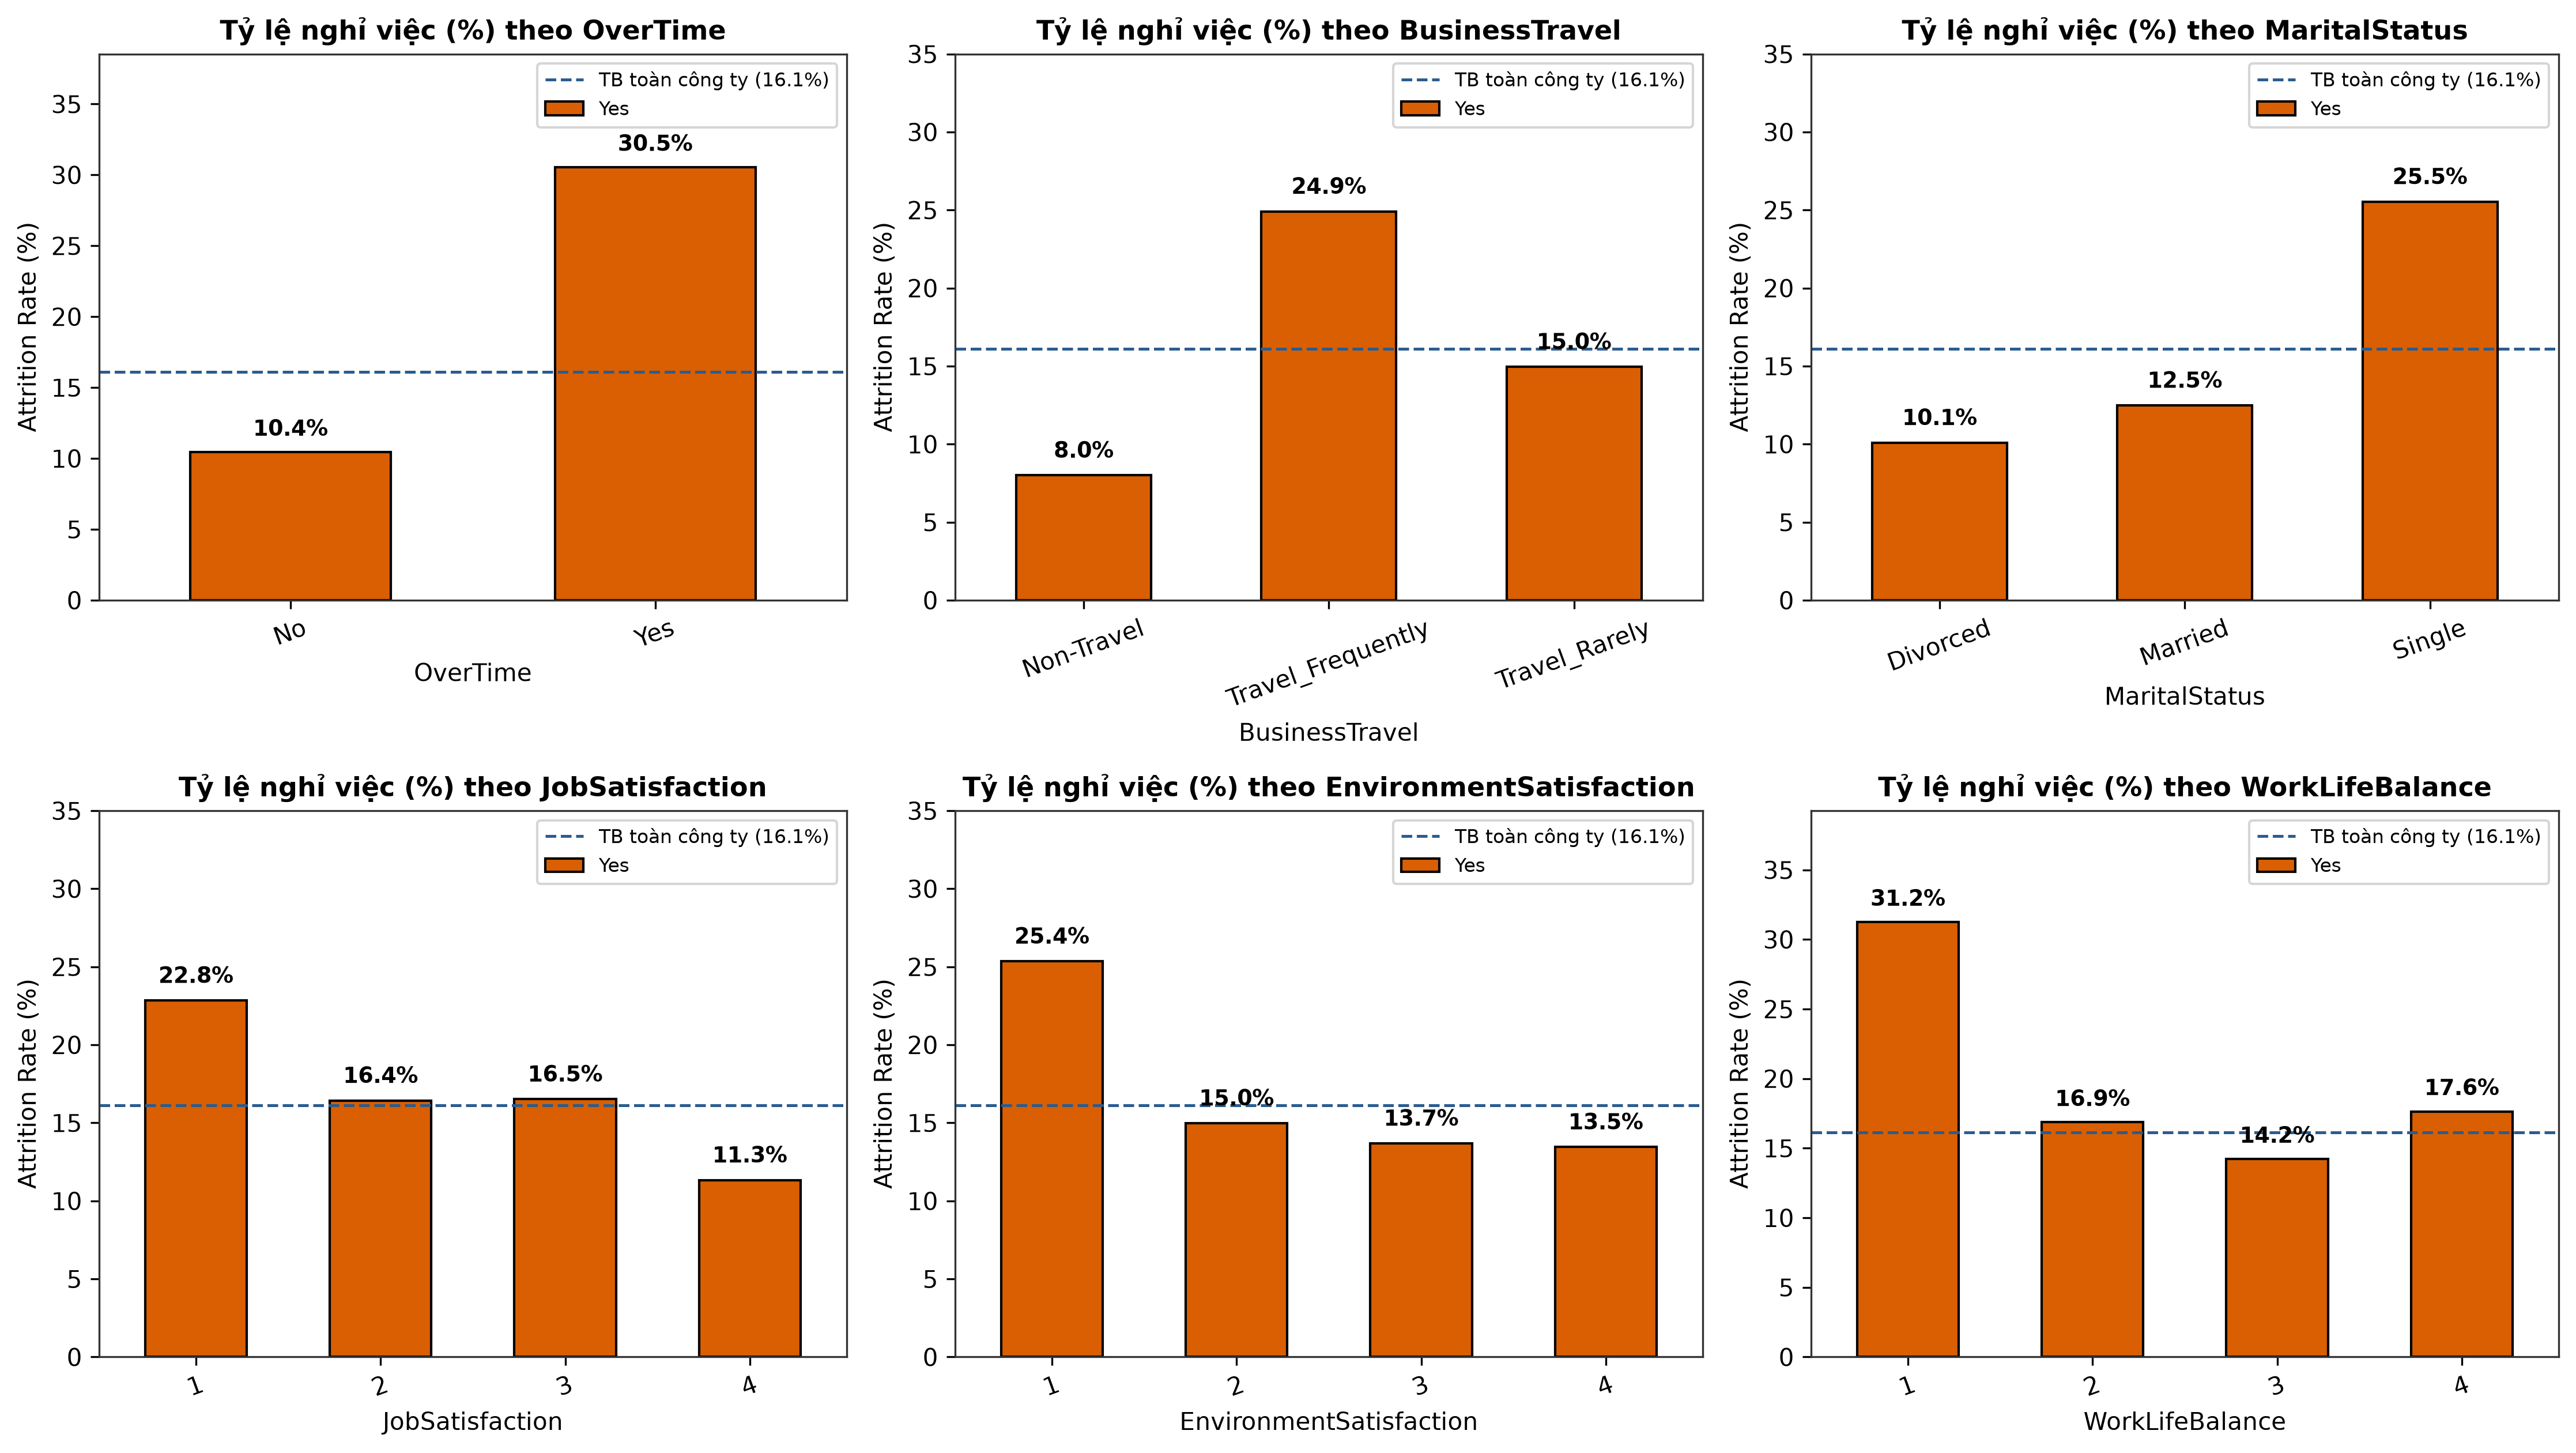
\includegraphics[width=0.98\textwidth]{figures/fig3_categorical_attrition.png}
    \caption{Tỷ lệ nghỉ việc (\%) theo các đặc trưng phân loại và thứ bậc trọng tâm.}
    \label{fig:cat_attrition}
\end{figure}

\subsubsection{Phân tích tương quan và kiểm tra nguy cơ rò rỉ dữ liệu (Data Leakage)}
Hình \ref{fig:corr_heatmap} trình bày ma trận tương quan Pearson giữa các biến số chính và biến mục tiêu \texttt{Attrition\_Num}.
\begin{itemize}
    \item \textbf{Đa cộng tuyến rất cao (\textit{Multicollinearity}):} Cặp biến \texttt{JobLevel} và \texttt{MonthlyIncome} có hệ số tương quan $r = \mathbf{0.95}$ (cấp bậc công việc và lương tháng gần như biểu diễn cùng một thông tin). Ngoài ra, cụm 4 biến thâm niên (\texttt{TotalWorkingYears}, \texttt{YearsAtCompany}, \texttt{YearsInCurrentRole}, \texttt{YearsWithCurrManager}) tương quan chặt chẽ với nhau ($r \in [0.63, 0.78]$).
    \item \textbf{Các biến nhiễu không mang thông tin:} Ba cột \texttt{DailyRate}, \texttt{HourlyRate}, \texttt{MonthlyRate} trong bộ dữ liệu giả lập của IBM hoàn toàn không có tương quan với \texttt{MonthlyIncome} ($|r| < 0.03$) lẫn \texttt{Attrition}, đóng vai trò như nhiễu ngẫu nhiên.
    \item \textbf{Đánh giá nguy cơ Data Leakage:} Toàn bộ 34 thuộc tính đầu vào đều là thông tin hồ sơ nhân sự được ghi nhận trước hoặc trong quá trình làm việc; không có cột nào chứa thông tin phát sinh sau sự kiện nghỉ việc.
\end{itemize}

\begin{figure}[H]
    \centering
    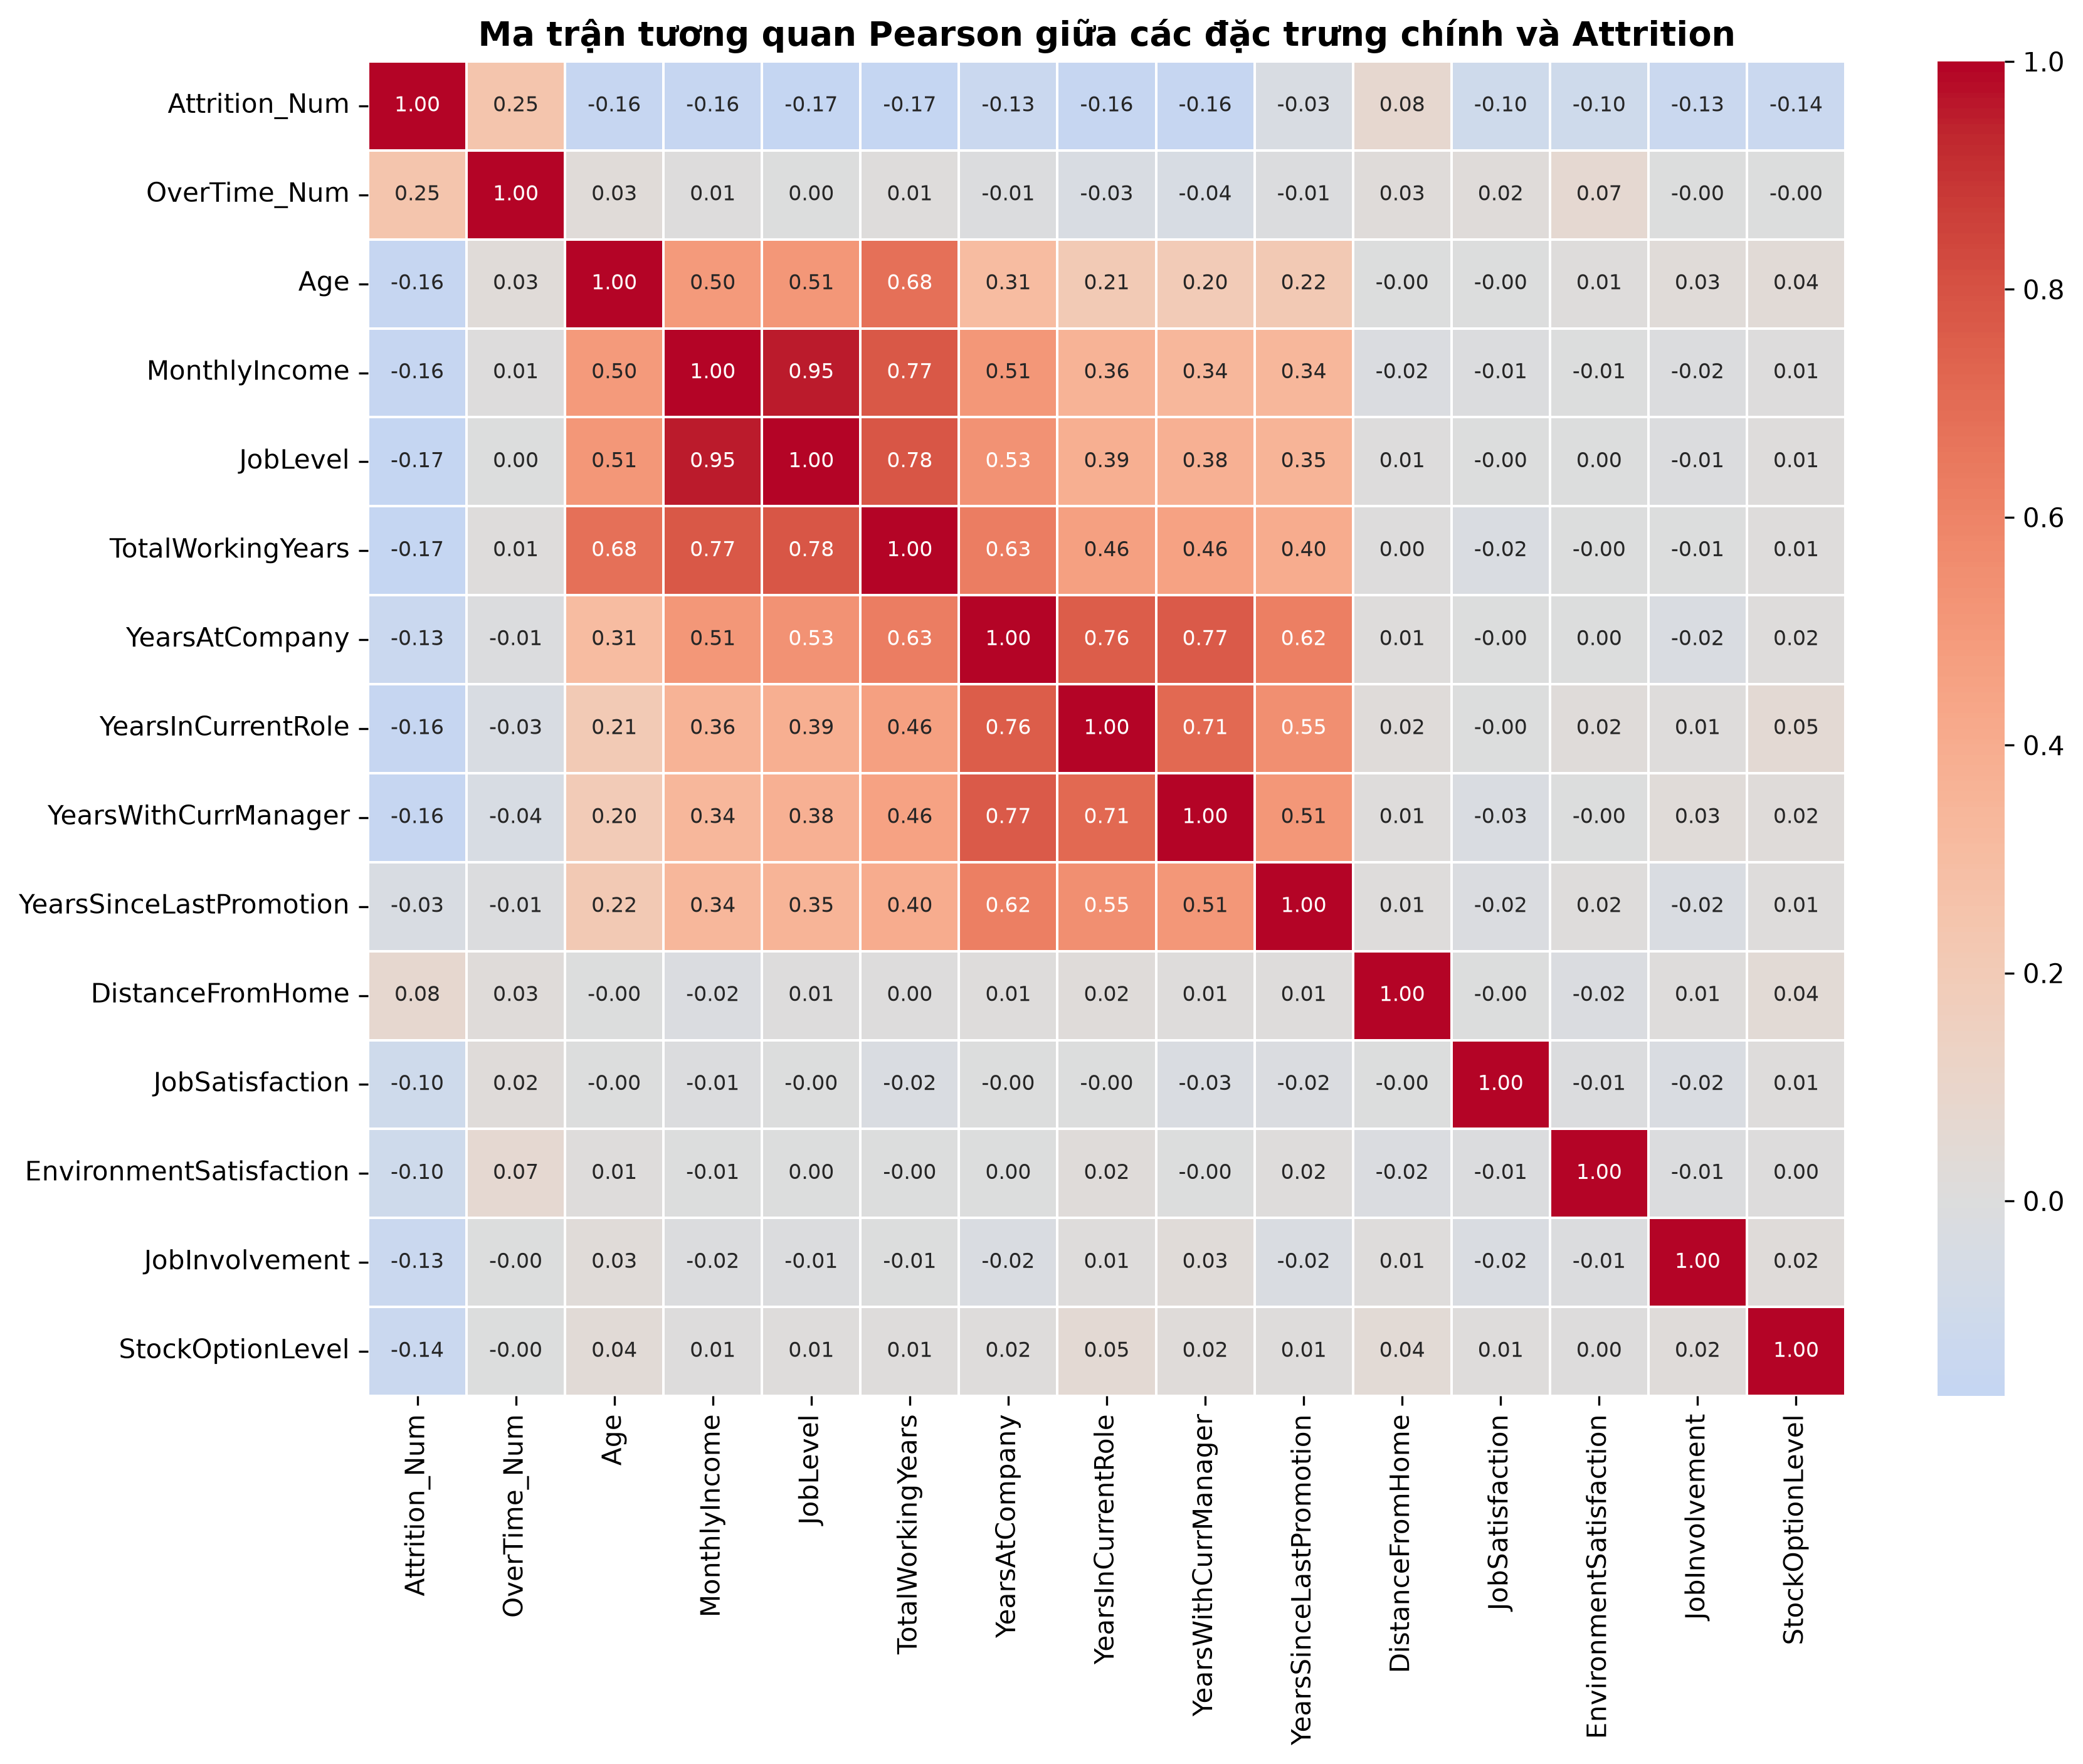
\includegraphics[width=0.90\textwidth]{figures/fig4_correlation_heatmap.png}
    \caption{Ma trận tương quan Pearson giữa các đặc trưng chính và nhãn \texttt{Attrition}.}
    \label{fig:corr_heatmap}
\end{figure}

% =====================================================================
% CHƯƠNG 2: THIẾT KẾ GIẢI PHÁP VÀ QUY TRÌNH HỌC MÁY
% =====================================================================
\section{Thiết kế giải pháp và quy trình học máy}

\subsection{Sơ đồ quy trình học máy tổng quát}
Quy trình thực hiện của nhóm tuân thủ chặt chẽ sơ đồ chuẩn của học phần, được thiết kế thành hai luồng xử lý song song (\textbf{Luồng A} và \textbf{Luồng B}) như minh họa trong Hình \ref{fig:pipeline_diagram}.

\begin{figure}[H]
\centering
\begin{tikzpicture}[
    node distance=1.0cm and 1.2cm,
    box/.style={rectangle, rounded corners=4pt, draw=blue!70!black, fill=blue!6, thick, minimum width=3.1cm, minimum height=1.0cm, align=center, font=\footnotesize\bfseries},
    streamA/.style={rectangle, rounded corners=4pt, draw=teal!80!black, fill=teal!8, thick, minimum width=5.6cm, minimum height=1.1cm, align=center, font=\footnotesize},
    streamB/.style={rectangle, rounded corners=4pt, draw=orange!85!black, fill=orange!10, thick, minimum width=5.6cm, minimum height=1.1cm, align=center, font=\footnotesize},
    arrow/.style={-{Stealth[length=2.5mm]}, thick, draw=black!75}
]
    \node[box] (data) {1. Dữ liệu thô\\(1470 $\times$ 35) \& EDA};
    \node[box, right=1.0cm of data] (split) {2. Chia Train/Test\\(80/20, Stratified,\\random\_state=42)};

    \node[streamA, below left=1.1cm and -1.5cm of split] (luongA) {\textbf{3A. Luồng A (Pipeline cơ bản)}\\Bỏ 4 cột ID/hằng số + \texttt{OneHotEncoder}\\+ \texttt{StandardScaler} (44 chiều)};
    \node[streamB, below right=1.1cm and -1.5cm of split] (luongB) {\textbf{3B. Luồng B (Pipeline cải tiến)}\\7 đặc trưng HR mới + $\log(1+x)$ + Bỏ nhiễu\\+ \texttt{RobustScaler} + \texttt{SelectKBest}};

    \node[box, below=2.8cm of split, minimum width=7.5cm] (models) {4. Huấn luyện \& Tinh chỉnh (\texttt{GridSearchCV} 5-Fold)\\Baseline (\texttt{Dummy}) $\mid$ \texttt{K-NN} $\mid$ \texttt{Gaussian NB} $\mid$ \texttt{Decision Tree} $\mid$ \texttt{Random Forest}};

    \node[box, below=0.9cm of models, minimum width=7.5cm] (eval) {5. Đánh giá (\texttt{Precision, Recall, F1, ROC-AUC, CM})\\\& Phân tích lỗi chuyên sâu (\textit{False Negatives / False Positives})};

    \draw[arrow] (data) -- (split);
    \draw[arrow] (split.south) -| (luongA.north);
    \draw[arrow] (split.south) -| (luongB.north);
    \draw[arrow] (luongA.south) |- ([yshift=0.2cm]models.north west) -- (models.north west);
    \draw[arrow] (luongB.south) |- ([yshift=0.2cm]models.north east) -- (models.north east);
    \draw[arrow] (models) -- (eval);
\end{tikzpicture}
\caption{Sơ đồ kiến trúc Pipeline học máy và hai luồng thử nghiệm (Luồng A \& Luồng B).}
\label{fig:pipeline_diagram}
\end{figure}

\subsection{Cách chia dữ liệu và cơ chế chống rò rỉ dữ liệu (Data Leakage)}
\begin{itemize}
    \item \textbf{Chia tập dữ liệu:} Bộ dữ liệu gốc ($1{,}470$ mẫu) được chia thành tập huấn luyện (\texttt{Train}: $80\%$, gồm $1{,}176$ mẫu với $190$ mẫu lớp \texttt{Yes} -- $16.16\%$) và tập kiểm thử (\texttt{Test}: $20\%$, gồm $294$ mẫu với $47$ mẫu lớp \texttt{Yes} -- $15.99\%$) bằng hàm \texttt{train\_test\_split(..., test\_size=0.20, stratify=y, random\_state=42)}.
    \item \textbf{Chống Data Leakage:} Toàn bộ các bước học tham số thống kê từ dữ liệu (trung bình/độ lệch chuẩn của \texttt{StandardScaler}, trung vị/IQR của \texttt{RobustScaler}, danh mục của \texttt{OneHotEncoder}, và điểm số F-value của \texttt{SelectKBest}) đều được đóng gói trong đối tượng \texttt{sklearn.pipeline.Pipeline}. Khi gọi \texttt{GridSearchCV} trên tập \texttt{Train}, các bộ biến đổi chỉ được \texttt{fit} trên các fold huấn luyện và \texttt{transform} trên fold kiểm định; tập \texttt{Test} hoàn toàn cô lập cho đến bước đánh giá cuối cùng.
\end{itemize}

\subsection{Thiết kế hai luồng tiền xử lý và kỹ thuật đặc trưng}
Để trả lời câu hỏi nghiên cứu \textit{``Thay đổi cách chuẩn bị dữ liệu có làm thay đổi hiệu quả mô hình hay không, và tại sao?''}, nhóm xây dựng hai cấu hình xử lý dữ liệu từ cùng một tập dữ liệu thô:

\subsubsection{Luồng A: Pipeline cơ bản (Basic Pipeline)}
\begin{enumerate}
    \item Loại bỏ 4 cột không mang thông tin dự đoán: \texttt{EmployeeNumber}, \texttt{EmployeeCount}, \texttt{Over18}, \texttt{StandardHours}.
    \item Mã hóa 7 biến phân loại kiểu chuỗi (\texttt{BusinessTravel}, \texttt{Department}, \texttt{EducationField}, \texttt{Gender}, \texttt{JobRole}, \texttt{MaritalStatus}, \texttt{OverTime}) bằng \texttt{OneHotEncoder(drop='first')}.
    \item Chuẩn hóa toàn bộ 23 biến số còn lại bằng \texttt{StandardScaler} ($z = \frac{x - \mu}{\sigma}$). Tổng số chiều đặc trưng sau biến đổi của Luồng A là $44$ chiều.
\end{enumerate}

\subsubsection{Luồng B: Pipeline cải tiến (Improved Pipeline)}
Dựa trên các phát hiện từ bước EDA, Luồng B thực hiện 4 cải tiến kỹ thuật quan trọng:
\begin{enumerate}
    \item \textbf{Tạo 7 đặc trưng mới có ý nghĩa nghiệp vụ nhân sự (HR Domain Features):}
    \begin{itemize}
        \item \texttt{PromotionStagnationRatio} $= \frac{\text{YearsSinceLastPromotion}}{\text{YearsAtCompany} + 1}$: Đo lường tỷ lệ thời gian bị chững lại không được thăng chức tại công ty.
        \item \texttt{CompanyTenureRatio} $= \frac{\text{YearsAtCompany}}{\text{TotalWorkingYears} + 1}$: Phản ánh mức độ gắn bó với công ty hiện tại so với toàn bộ sự nghiệp.
        \item \texttt{IncomePerWorkingYear} $= \frac{\text{MonthlyIncome}}{\text{TotalWorkingYears} + 1}$: Mức thu nhập đạt được trên mỗi năm kinh nghiệm.
        \item \texttt{OverallSatisfaction} $= \frac{1}{4}(\text{EnvSat} + \text{JobSat} + \text{RelSat} + \text{WorkLifeBalance})$: Chỉ số hài lòng tổng hợp trên 4 khía cạnh.
        \item \texttt{RoleStabilityRatio} $= \frac{\text{YearsInCurrentRole}}{\text{YearsAtCompany} + 1}$: Tỷ lệ ổn định ở vị trí công việc hiện tại.
        \item \texttt{OverTime\_FrequentTravel}: Biến nhị phân tương tác nhận giá trị $1$ khi nhân viên vừa phải làm thêm giờ (\texttt{OverTime = Yes}) vừa phải đi công tác thường xuyên (\texttt{Travel\_Frequently}).
        \item \texttt{YoungSingleLowIncome}: Biến nhị phân nhận diện nhóm nguy cơ cao (nhân viên dưới $30$ tuổi, độc thân và lương tháng dưới $\$3{,}500$).
    \end{itemize}
    \item \textbf{Mã hóa thứ bậc tự nhiên (\textit{Ordinal Encoding}):} Chuyển biến \texttt{BusinessTravel} thành biến thứ bậc \texttt{BusinessTravel\_Ord} $\in \{0, 1, 2\}$ phản ánh đúng cường độ đi lại tăng dần.
    \item \textbf{Xử lý phân phối lệch phải và ngoại lệ:} Áp dụng phép biến đổi $\log(1 + x)$ (\texttt{np.log1p}) cho 5 biến liên tục lệch phải mạnh (\texttt{MonthlyIncome}, \texttt{TotalWorkingYears}, \texttt{YearsAtCompany}, \texttt{YearsSinceLastPromotion}, \texttt{DistanceFromHome}) để kéo phân phối về gần dạng chuẩn, sau đó chuẩn hóa bằng \texttt{RobustScaler} ($z_{\text{robust}} = \frac{x - \text{Median}}{\text{IQR}}$) giúp giảm ảnh hưởng của các điểm ngoại lệ.
    \item \textbf{Loại bỏ biến đa cộng tuyến/nhiễu và chọn lọc đặc trưng:} Loại bỏ cột \texttt{JobLevel} (tương quan $0.95$ với \texttt{MonthlyIncome}) và 3 cột nhiễu ngẫu nhiên (\texttt{DailyRate}, \texttt{HourlyRate}, \texttt{MonthlyRate}), đồng thời tích hợp bước chọn lọc đặc trưng \texttt{SelectKBest(f\_classif)} cho K-NN và Naive Bayes.
\end{enumerate}

Hình \ref{fig:eng_features} trực quan hóa khả năng phân tách hai lớp \texttt{Yes}/\texttt{No} của các đặc trưng mới được tạo trong Luồng B. Có thể thấy nhóm nhân viên có $\texttt{OverTime\_FrequentTravel} = 1$ có tỷ lệ nghỉ việc vọt lên tới $\mathbf{56.1\%}$ (gấp $3.5$ lần trung bình công ty), và nhóm $\texttt{YoungSingleLowIncome} = 1$ có tỷ lệ nghỉ việc $\mathbf{43.9\%}$.

\begin{figure}[H]
    \centering
    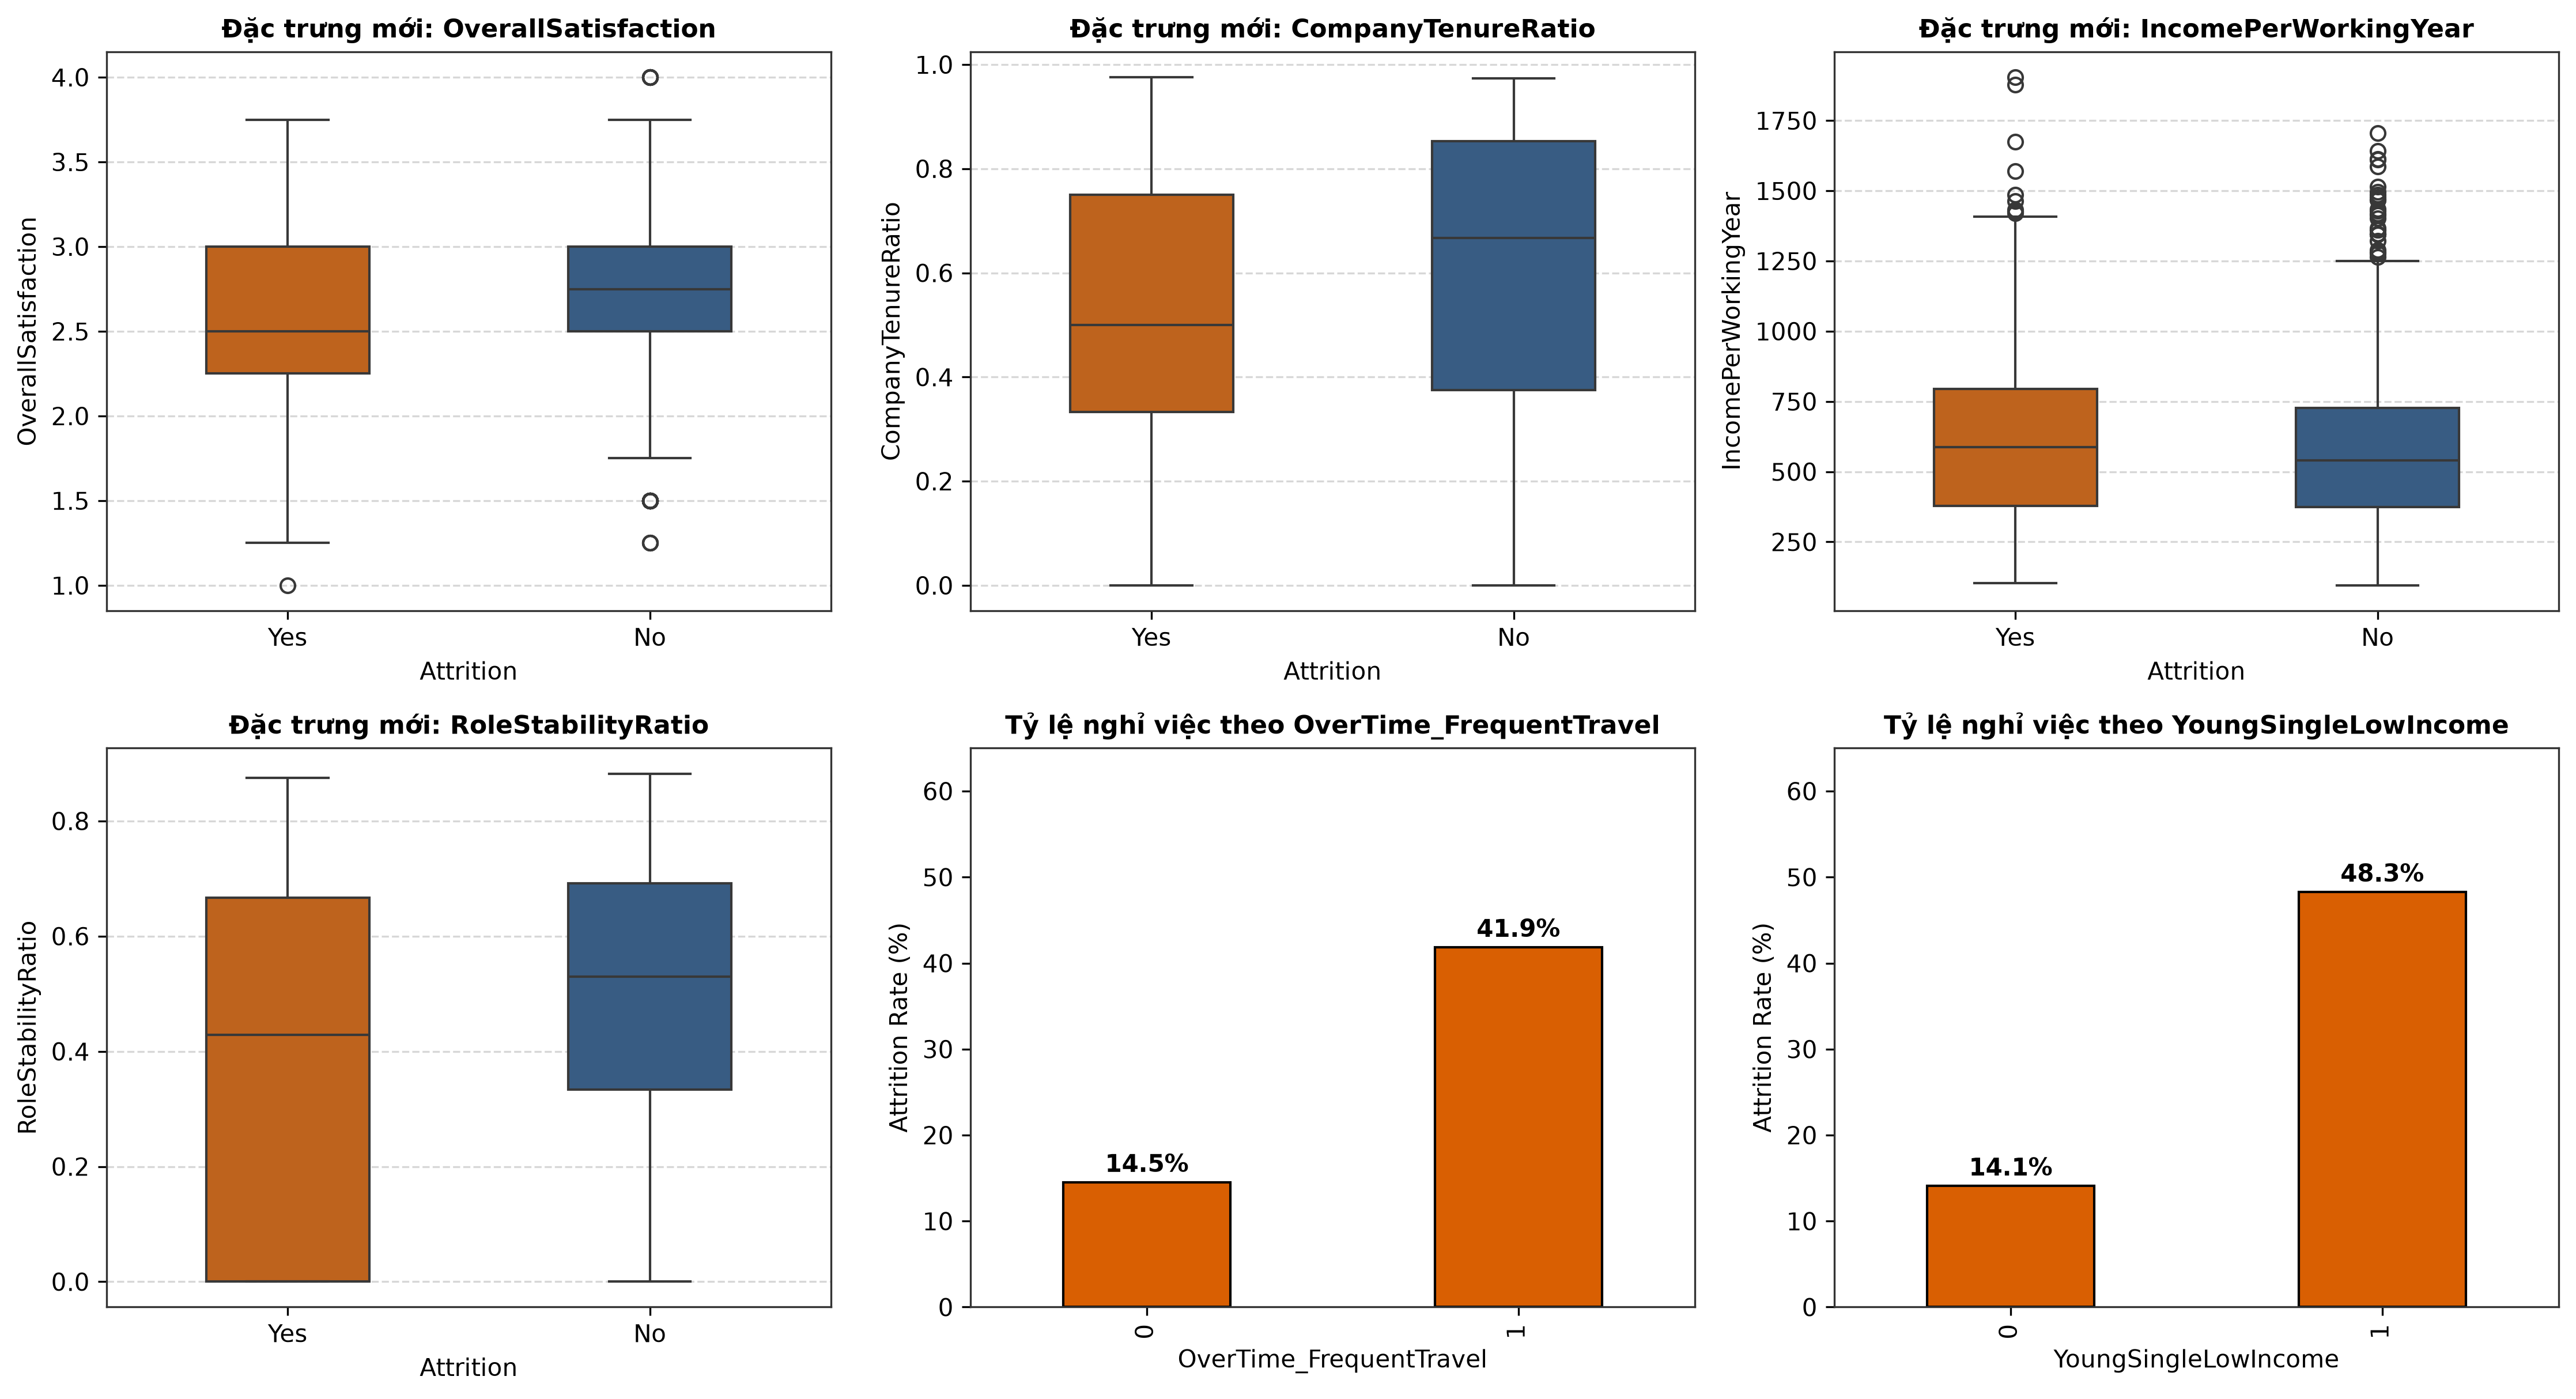
\includegraphics[width=0.98\textwidth]{figures/fig11_engineered_features.png}
    \caption{Trực quan hóa sự phân tách lớp của các đặc trưng nghiệp vụ HR mới tạo trong Luồng B.}
    \label{fig:eng_features}
\end{figure}

\subsection{Mô tả các thuật toán học máy được lựa chọn}
Nhóm lựa chọn đầy đủ 3 thuật toán phân loại đã học trong học phần cùng 1 thuật toán mở rộng:
\begin{enumerate}
    \item \textbf{K-Nearest Neighbors (K-NN):} Phân loại một mẫu mới dựa trên biểu quyết đa số (hoặc có trọng số nghịch đảo khoảng cách) của $k$ láng giềng gần nhất trong không gian đặc trưng theo khoảng cách Minkowski ($p=2$: Euclidean, $p=1$: Manhattan). K-NN rất nhạy cảm với thang đo đặc trưng và số chiều không gian lớn (\textit{curse of dimensionality}).
    \item \textbf{Gaussian Naive Bayes (Gaussian NB):} Áp dụng định lý Bayes với giả định các đặc trưng độc lập có điều kiện khi biết nhãn lớp và mỗi đặc trưng liên tục tuân theo phân phối chuẩn $P(x_j \mid y=c) = \frac{1}{\sqrt{2\pi\sigma_{jc}^2}}\exp\left(-\frac{(x_j - \mu_{jc})^2}{2\sigma_{jc}^2}\right)$. Tham số \texttt{var\_smoothing} cộng thêm một tỷ lệ phương sai lớn nhất vào mọi phương sai đặc trưng để ổn định số học và làm mượt biên quyết định.
    \item \textbf{Cây quyết định (Decision Tree):} Chia đệ quy không gian đặc trưng bằng các siêu phẳng song song với trục tọa độ nhằm cực đại hóa độ giảm độ vẩn đục (\textit{Impurity}) theo chỉ số \texttt{Gini} ($1 - \sum_c p_c^2$) hoặc \texttt{Entropy} ($-\sum_c p_c \log_2 p_c$). Để chống học vẹt (\textit{overfitting}) và xử lý mất cân bằng lớp, các tham số \texttt{max\_depth}, \texttt{min\_samples\_leaf} và \texttt{class\_weight='balanced'} đóng vai trò quyết định.
    \item \textbf{Random Forest (Kỹ thuật mở rộng):} Mô hình học kết hợp (\textit{Ensemble Bagging}) xây dựng $200$ cây quyết định trên các mẫu bootstrap và tập con đặc trưng ngẫu nhiên, giúp giảm phương sai của cây quyết định đơn lẻ.
\end{enumerate}

% =====================================================================
% CHƯƠNG 3: PHÂN TÍCH MÃ NGUỒN VÀ CHỨC NĂNG
% =====================================================================
\section{Phân tích mã nguồn và chức năng}

\subsection{Cấu trúc chương trình và tổ chức Notebook}
Mã nguồn của dự án được tổ chức theo cấu trúc chuẩn hóa, dễ tái lập như sau:
\begin{itemize}
    \item \texttt{data/WA\_Fn-UseC\_-HR-Employee-Attrition.csv}: Tập dữ liệu gốc của Đề tài 13.
    \item \texttt{notebooks/DeTai13\_Employee\_Attrition.ipynb}: Notebook chính thực hiện toàn bộ quy trình từ EDA, tiền xử lý hai luồng A/B, huấn luyện, tinh chỉnh tham số đến phân tích lỗi và tự động xuất biểu đồ độ phân giải cao.
    \item \texttt{report/main.tex}, \texttt{report/references.bib}, \texttt{report/figures/}: Mã nguồn báo cáo \LaTeX{} và các biểu đồ thực nghiệm.
    \item \texttt{README.md}, \texttt{requirements.txt}, \texttt{AI\_USAGE.md}: Tài liệu hướng dẫn chạy chương trình, khai báo thư viện và khai báo sử dụng AI.
\end{itemize}

\subsection{Các đoạn mã nguồn cốt lõi}
Thay vì chèn toàn bộ mã nguồn, phần này trích dẫn 2 đoạn mã quan trọng nhất thể hiện kỹ thuật thiết kế Pipeline chống rò rỉ dữ liệu của nhóm. Đoạn mã \ref{lst:fe_transformer} trình bày bộ biến đổi \texttt{HRFeatureEngineer} trong Luồng B.

\begin{lstlisting}[caption={Lớp biến đổi đặc trưng tùy chỉnh \texttt{HRFeatureEngineer} cho Luồng B.}, label={lst:fe_transformer}]
class HRFeatureEngineer(BaseEstimator, TransformerMixin):
    def __init__(self, drop_collinear=True):
        self.drop_collinear = drop_collinear

    def fit(self, X, y=None):
        return self

    def transform(self, X):
        X_out = X.copy()
        for c in ['EmployeeCount', 'Over18', 'StandardHours', 'EmployeeNumber']:
            if c in X_out.columns:
                X_out = X_out.drop(columns=[c])

        # 1. Tao 7 dac trung nghiep vu HR (Domain Features)
        X_out['PromotionStagnationRatio'] = X_out['YearsSinceLastPromotion'] / (X_out['YearsAtCompany'] + 1.0)
        X_out['CompanyTenureRatio'] = X_out['YearsAtCompany'] / (X_out['TotalWorkingYears'] + 1.0)
        X_out['IncomePerWorkingYear'] = X_out['MonthlyIncome'] / (X_out['TotalWorkingYears'] + 1.0)
        X_out['OverallSatisfaction'] = (
            X_out['EnvironmentSatisfaction'] + X_out['JobSatisfaction'] +
            X_out['RelationshipSatisfaction'] + X_out['WorkLifeBalance']
        ) / 4.0
        X_out['RoleStabilityRatio'] = X_out['YearsInCurrentRole'] / (X_out['YearsAtCompany'] + 1.0)
        X_out['OverTime_FrequentTravel'] = (
            (X_out['OverTime'] == 'Yes') & (X_out['BusinessTravel'] == 'Travel_Frequently')
        ).astype(int)
        X_out['YoungSingleLowIncome'] = (
            (X_out['Age'] < 30) & (X_out['MaritalStatus'] == 'Single') & (X_out['MonthlyIncome'] < 3500)
        ).astype(int)

        # 2. Ma hoa thu bac BusinessTravel va bien doi log1p cho bien lech phai
        travel_map = {'Non-Travel': 0, 'Travel_Rarely': 1, 'Travel_Frequently': 2}
        X_out['BusinessTravel_Ord'] = X_out['BusinessTravel'].map(travel_map).fillna(1)
        X_out = X_out.drop(columns=['BusinessTravel'])

        for col in ['MonthlyIncome', 'TotalWorkingYears', 'YearsAtCompany', 'YearsSinceLastPromotion', 'DistanceFromHome']:
            X_out[col] = np.log1p(np.maximum(0, X_out[col]))

        if self.drop_collinear:
            X_out = X_out.drop(columns=['JobLevel', 'DailyRate', 'HourlyRate', 'MonthlyRate'])
        return X_out
\end{lstlisting}

Đoạn mã \ref{lst:gridsearch} minh họa cách kết hợp \texttt{Pipeline}, \texttt{SelectKBest} và \texttt{GridSearchCV} tối ưu theo thước đo \texttt{F1-score} trên các fold phân tầng.

\begin{lstlisting}[caption={Đóng gói Pipeline và tìm kiếm siêu tham số bằng \texttt{GridSearchCV}.}, label={lst:gridsearch}]
cv = StratifiedKFold(n_splits=5, shuffle=True, random_state=42)

pipe_dt = Pipeline([
    ('prep', preprocessor_B),
    ('clf', DecisionTreeClassifier(random_state=42))
])
param_grid_dt = {
    'clf__criterion': ['gini', 'entropy'],
    'clf__max_depth': [3, 4, 5, 6, 8, 10, None],
    'clf__min_samples_leaf': [5, 10, 15, 20],
    'clf__class_weight': [None, 'balanced']
}
gs_dt = GridSearchCV(pipe_dt, param_grid_dt, cv=cv, scoring='f1', n_jobs=1)
gs_dt.fit(X_train, y_train)
\end{lstlisting}

% =====================================================================
% CHƯƠNG 4: THỬ NGHIỆM VÀ KẾT QUẢ
% =====================================================================
\section{Thử nghiệm và kết quả}

\subsection{Thiết lập thí nghiệm và tiêu chí đánh giá}
Trên tập kiểm thử độc lập gồm $294$ mẫu ($247$ mẫu lớp \texttt{No} và $47$ mẫu lớp \texttt{Yes}), nhóm đánh giá mọi phương án qua 5 độ đo:
\begin{itemize}
    \item \textbf{Accuracy:} Tỷ lệ dự đoán đúng trên toàn bộ tập kiểm thử $\frac{TP + TN}{TP + TN + FP + FN}$. (Chỉ mang tính tham khảo do mất cân bằng lớp).
    \item \textbf{Precision (Lớp Yes):} $\frac{TP}{TP + FP}$ -- Trong số các nhân viên được mô hình cảnh báo sẽ nghỉ việc, có bao nhiêu phần trăm thực sự nghỉ việc.
    \item \textbf{Recall (Sensitivity -- Lớp Yes):} $\frac{TP}{TP + FN}$ -- Trong tổng số $47$ nhân viên thực sự nghỉ việc, mô hình phát hiện sớm được bao nhiêu phần trăm. Đây là chỉ số sống còn để không bỏ lỡ nhân sự cần giữ chân.
    \item \textbf{F1-score (Lớp Yes):} Trung bình điều hòa $F_1 = \frac{2 \cdot \text{Precision} \cdot \text{Recall}}{\text{Precision} + \text{Recall}}$, là tiêu chí chính để lựa chọn mô hình tối ưu trong \texttt{GridSearchCV}.
    \item \textbf{ROC-AUC:} Diện tích dưới đường cong ROC, đo khả năng phân tách hai lớp ở mọi ngưỡng xác suất.
\end{itemize}

\subsection{Phương án Baseline và kết quả các cấu hình tham số}
Nhóm thiết lập hai mốc \textbf{Baseline}:
\begin{enumerate}
    \item \textbf{Dummy Baseline:} \texttt{DummyClassifier(strategy='most\_frequent')} đạt $\text{Accuracy} = 84.01\%$ nhưng $\text{Recall} = 0.00\%, F_1 = 0.0000$; \texttt{DummyClassifier(strategy='stratified')} đạt $F_1 = 0.1250, \text{ROC-AUC} = 0.4768$.
    \item \textbf{Default Models trên Luồng A:} Chạy 3 thuật toán \texttt{K-NN}, \texttt{Gaussian NB}, \texttt{Decision Tree} với tham số mặc định của \texttt{scikit-learn} trên Luồng A.
\end{enumerate}

Sau khi thực hiện \texttt{GridSearchCV} 5-fold, bộ siêu tham số tối ưu tìm được cho từng mô hình như sau:
\begin{itemize}
    \item \textbf{K-NN (Luồng A):} \texttt{select\_\_k = 15, n\_neighbors = 3, metric = 'manhattan', weights = 'uniform'}.
    \item \textbf{K-NN (Luồng B):} \texttt{select\_\_k = 15, n\_neighbors = 3, metric = 'euclidean', weights = 'uniform'}.
    \item \textbf{Gaussian NB (Luồng A):} \texttt{select\_\_k = 30, var\_smoothing = 0.3162}.
    \item \textbf{Gaussian NB (Luồng B):} \texttt{select\_\_k = 'all', var\_smoothing = 0.0316}.
    \item \textbf{Decision Tree (Luồng A):} \texttt{criterion = 'entropy', max\_depth = 5, min\_samples\_leaf = 20, class\_weight = 'balanced'}.
    \item \textbf{Decision Tree (Luồng B):} \texttt{criterion = 'gini', max\_depth = 4, min\_samples\_leaf = 15, class\_weight = 'balanced'}.
\end{itemize}

Bảng \ref{tab:main_results} tổng hợp toàn bộ kết quả thực nghiệm trên tập kiểm thử ($294$ mẫu).

\begin{table}[H]
\centering
\caption{Bảng tổng hợp kết quả đánh giá trên 5-Fold Cross-Validation (Train) và Tập kiểm thử ($N_{\text{test}} = 294$).}
\label{tab:main_results}
\scriptsize
\begin{tabular}{l l l c c c c c c c}
\toprule
\textbf{Mô hình} & \textbf{Luồng} & \textbf{Giai đoạn} & \textbf{CV F1} & \textbf{Accuracy} & \textbf{Precision} & \textbf{Recall} & \textbf{Test F1} & \textbf{ROC-AUC} & \textbf{CM} $[[\text{TN, FP}], [\text{FN, TP}]]$ \\
\midrule
Dummy (Most Freq) & Luồng A & Baseline & 0.0000 & 0.8401 & 0.0000 & 0.0000 & 0.0000 & 0.5000 & $[[247, 0], [47, 0]]$ \\
Dummy (Stratified) & Luồng A & Baseline & 0.1644 & 0.7143 & 0.1224 & 0.1277 & 0.1250 & 0.4768 & $[[204, 43], [41, 6]]$ \\
\midrule
K-NN & Luồng A & Default & 0.2264 & 0.8367 & 0.4545 & 0.1064 & 0.1724 & 0.6181 & $[[241, 6], [42, 5]]$ \\
Gaussian NB & Luồng A & Default & 0.3902 & 0.6156 & 0.2500 & \textbf{0.7021} & 0.3687 & 0.6956 & $[[148, 99], [14, 33]]$ \\
Decision Tree & Luồng A & Default & 0.3714 & 0.7585 & 0.2931 & 0.3617 & 0.3238 & 0.5979 & $[[206, 41], [30, 17]]$ \\
\midrule
K-NN & Luồng B & Default & 0.2924 & \textbf{0.8503} & \textbf{0.6364} & 0.1489 & 0.2414 & 0.6285 & $[[243, 4], [40, 7]]$ \\
Gaussian NB & Luồng B & Default & 0.4304 & 0.7449 & 0.3444 & 0.6596 & 0.4526 & 0.7373 & $[[188, 59], [16, 31]]$ \\
Decision Tree & Luồng B & Default & 0.3257 & 0.7891 & 0.3529 & 0.3830 & 0.3673 & 0.6247 & $[[214, 33], [29, 18]]$ \\
\midrule
K-NN & Luồng A & Tuned & 0.3719 & 0.8469 & 0.5625 & 0.1915 & 0.2857 & 0.6677 & $[[240, 7], [38, 9]]$ \\
Gaussian NB & Luồng A & Tuned & 0.5029 & 0.7891 & 0.3729 & 0.4681 & 0.4151 & 0.7258 & $[[210, 37], [25, 22]]$ \\
Decision Tree & Luồng A & Tuned & 0.4438 & 0.7449 & 0.3409 & 0.6383 & 0.4444 & 0.7026 & $[[189, 58], [17, 30]]$ \\
Random Forest (Mở rộng) & Luồng A & Tuned & 0.4899 & 0.7993 & 0.4091 & 0.5745 & 0.4779 & \textbf{0.7819} & $[[208, 39], [20, 27]]$ \\
\midrule
\textbf{K-NN} & \textbf{Luồng B} & \textbf{Tuned} & 0.3498 & 0.8333 & 0.4615 & 0.2553 & \textbf{0.3288} & 0.6562 & $[[233, 14], [35, 12]]$ \\
\textbf{Gaussian NB} & \textbf{Luồng B} & \textbf{Tuned} & 0.5012 & 0.8027 & 0.4154 & 0.5745 & \textbf{0.4821} & \textbf{0.7507} & $[[209, 38], [20, 27]]$ \\
\textbf{Decision Tree} & \textbf{Luồng B} & \textbf{Tuned} & 0.4457 & 0.7279 & 0.3299 & \textbf{0.6809} & \textbf{0.4444} & 0.6972 & $[[182, 65], [15, 32]]$ \\
\textbf{Random Forest (Mở rộng)} & \textbf{Luồng B} & \textbf{Tuned} & \textbf{0.5056} & 0.8129 & 0.4394 & 0.6170 & \textbf{0.5133} & 0.7785 & $[[210, 37], [18, 29]]$ \\
\bottomrule
\end{tabular}
\end{table}

\subsection{Trực quan hóa kết quả thực nghiệm}

Hình \ref{fig:hyperparam_tuning} biểu diễn sự biến thiên của \texttt{F1-score} khi thay đổi số láng giềng $k$ của K-NN và độ sâu tối đa \texttt{max\_depth} của Cây quyết định trên cả hai luồng dữ liệu. Với K-NN, khi $k$ tăng lớn ($k \ge 11$), láng giềng thuộc lớp đa số (\texttt{No} -- $83.9\%$) áp đảo hoàn toàn khiến \texttt{F1-score} giảm mạnh; giá trị $k \in \{3, 5\}$ kết hợp chọn lọc đặc trưng ở Luồng B cho kết quả vượt trội so với Luồng A. Với Decision Tree, độ sâu \texttt{max\_depth} $\in \{3, 4, 5\}$ kết hợp \texttt{class\_weight='balanced'} giúp đạt đỉnh \texttt{F1-score}, trong khi tăng độ sâu quá lớn ($\ge 10$) làm cây học vẹt nhiễu và giảm hiệu năng.

\begin{figure}[H]
    \centering
    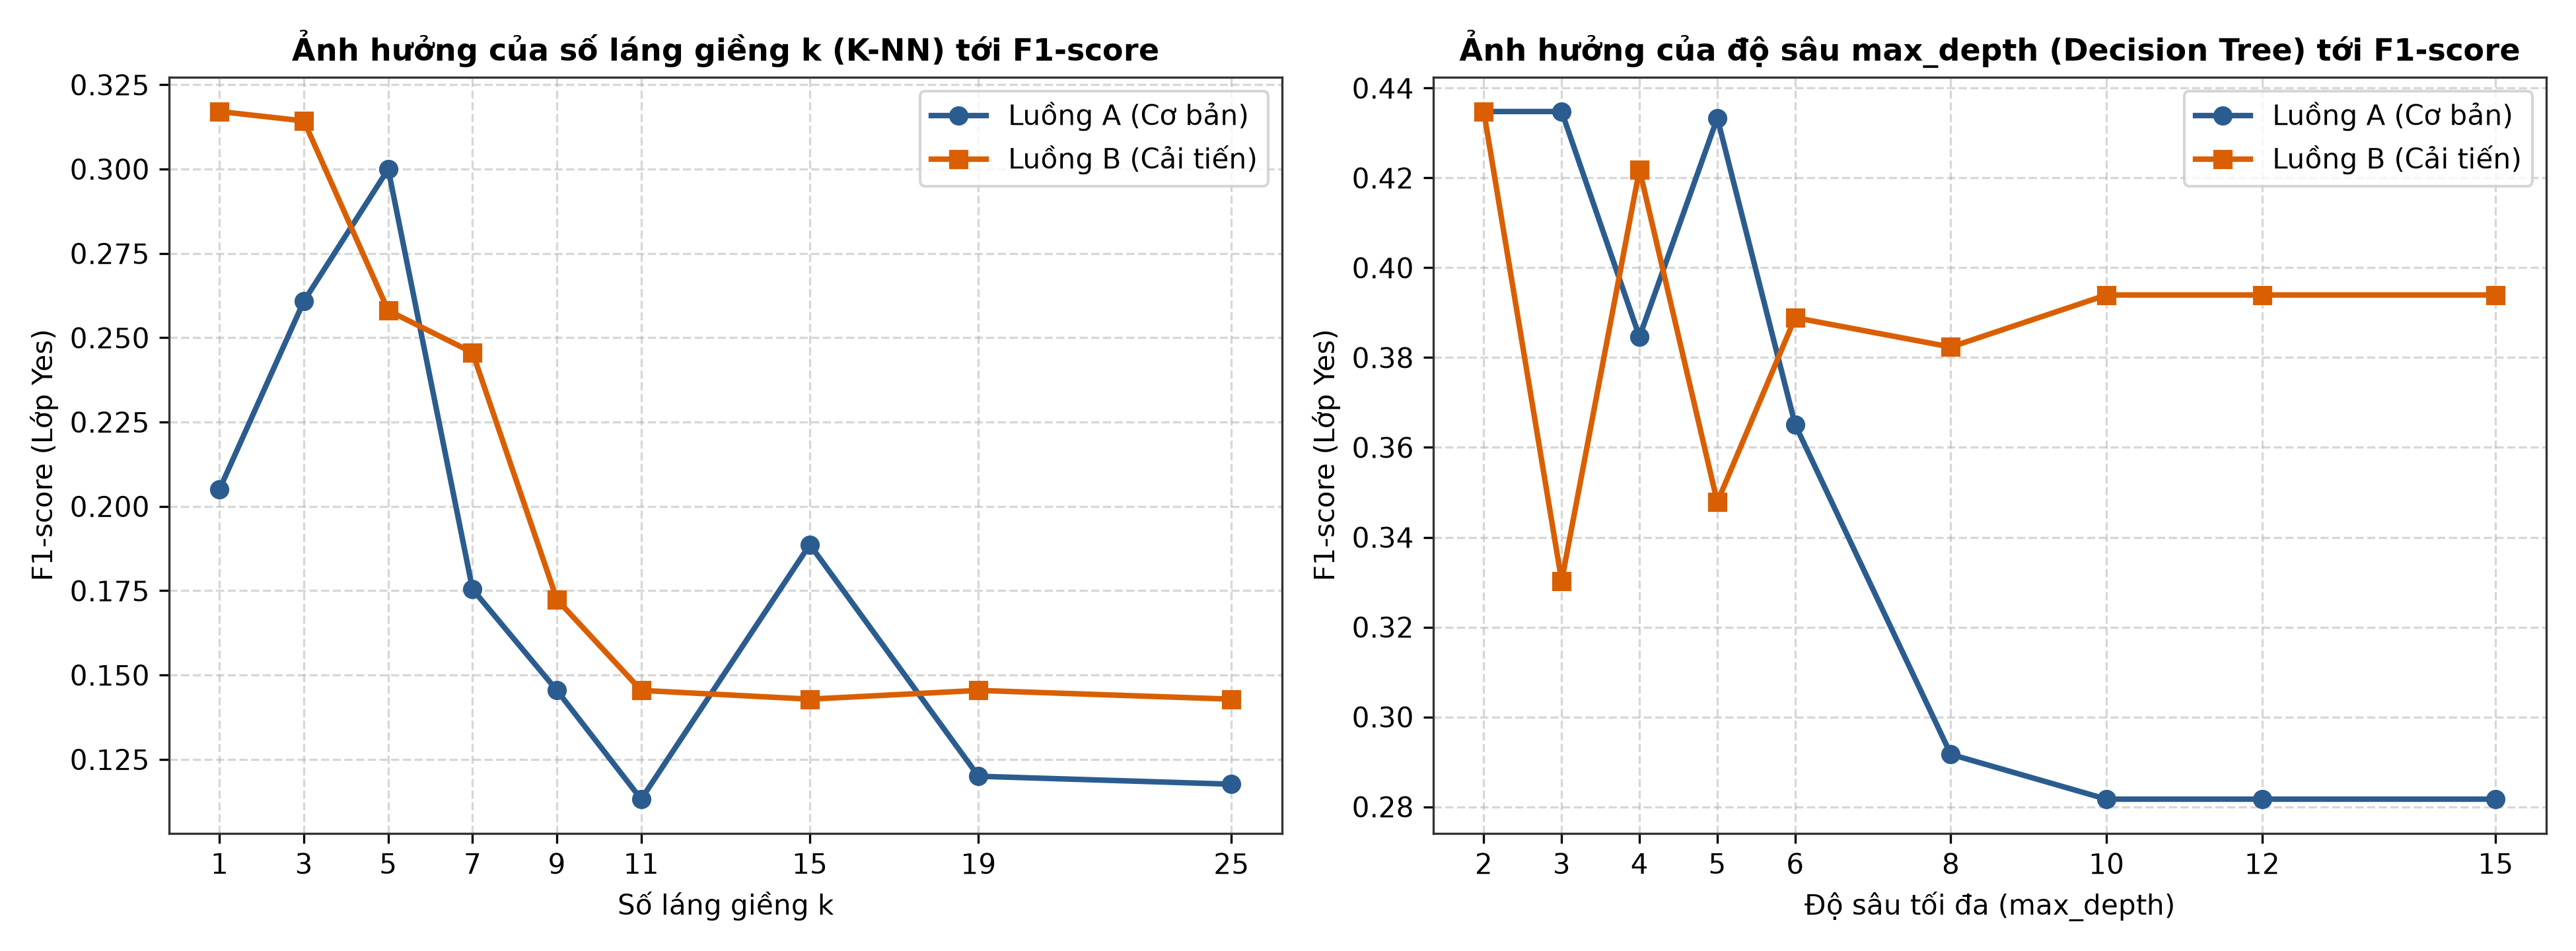
\includegraphics[width=0.98\textwidth]{figures/fig5_hyperparameter_tuning.png}
    \caption{Ảnh hưởng của siêu tham số $k$ (K-NN) và \texttt{max\_depth} (Decision Tree) tới F1-score.}
    \label{fig:hyperparam_tuning}
\end{figure}

Hình \ref{fig:model_comp} trực quan hóa sự cải thiện giữa Luồng A và Luồng B của các mô hình sau tinh chỉnh. Hình \ref{fig:cm_plot} và Hình \ref{fig:roc_plot} lần lượt trình bày Ma trận nhầm lẫn (\textit{Confusion Matrix}) và Đường cong ROC của các mô hình trên Luồng B.

\begin{figure}[H]
    \centering
    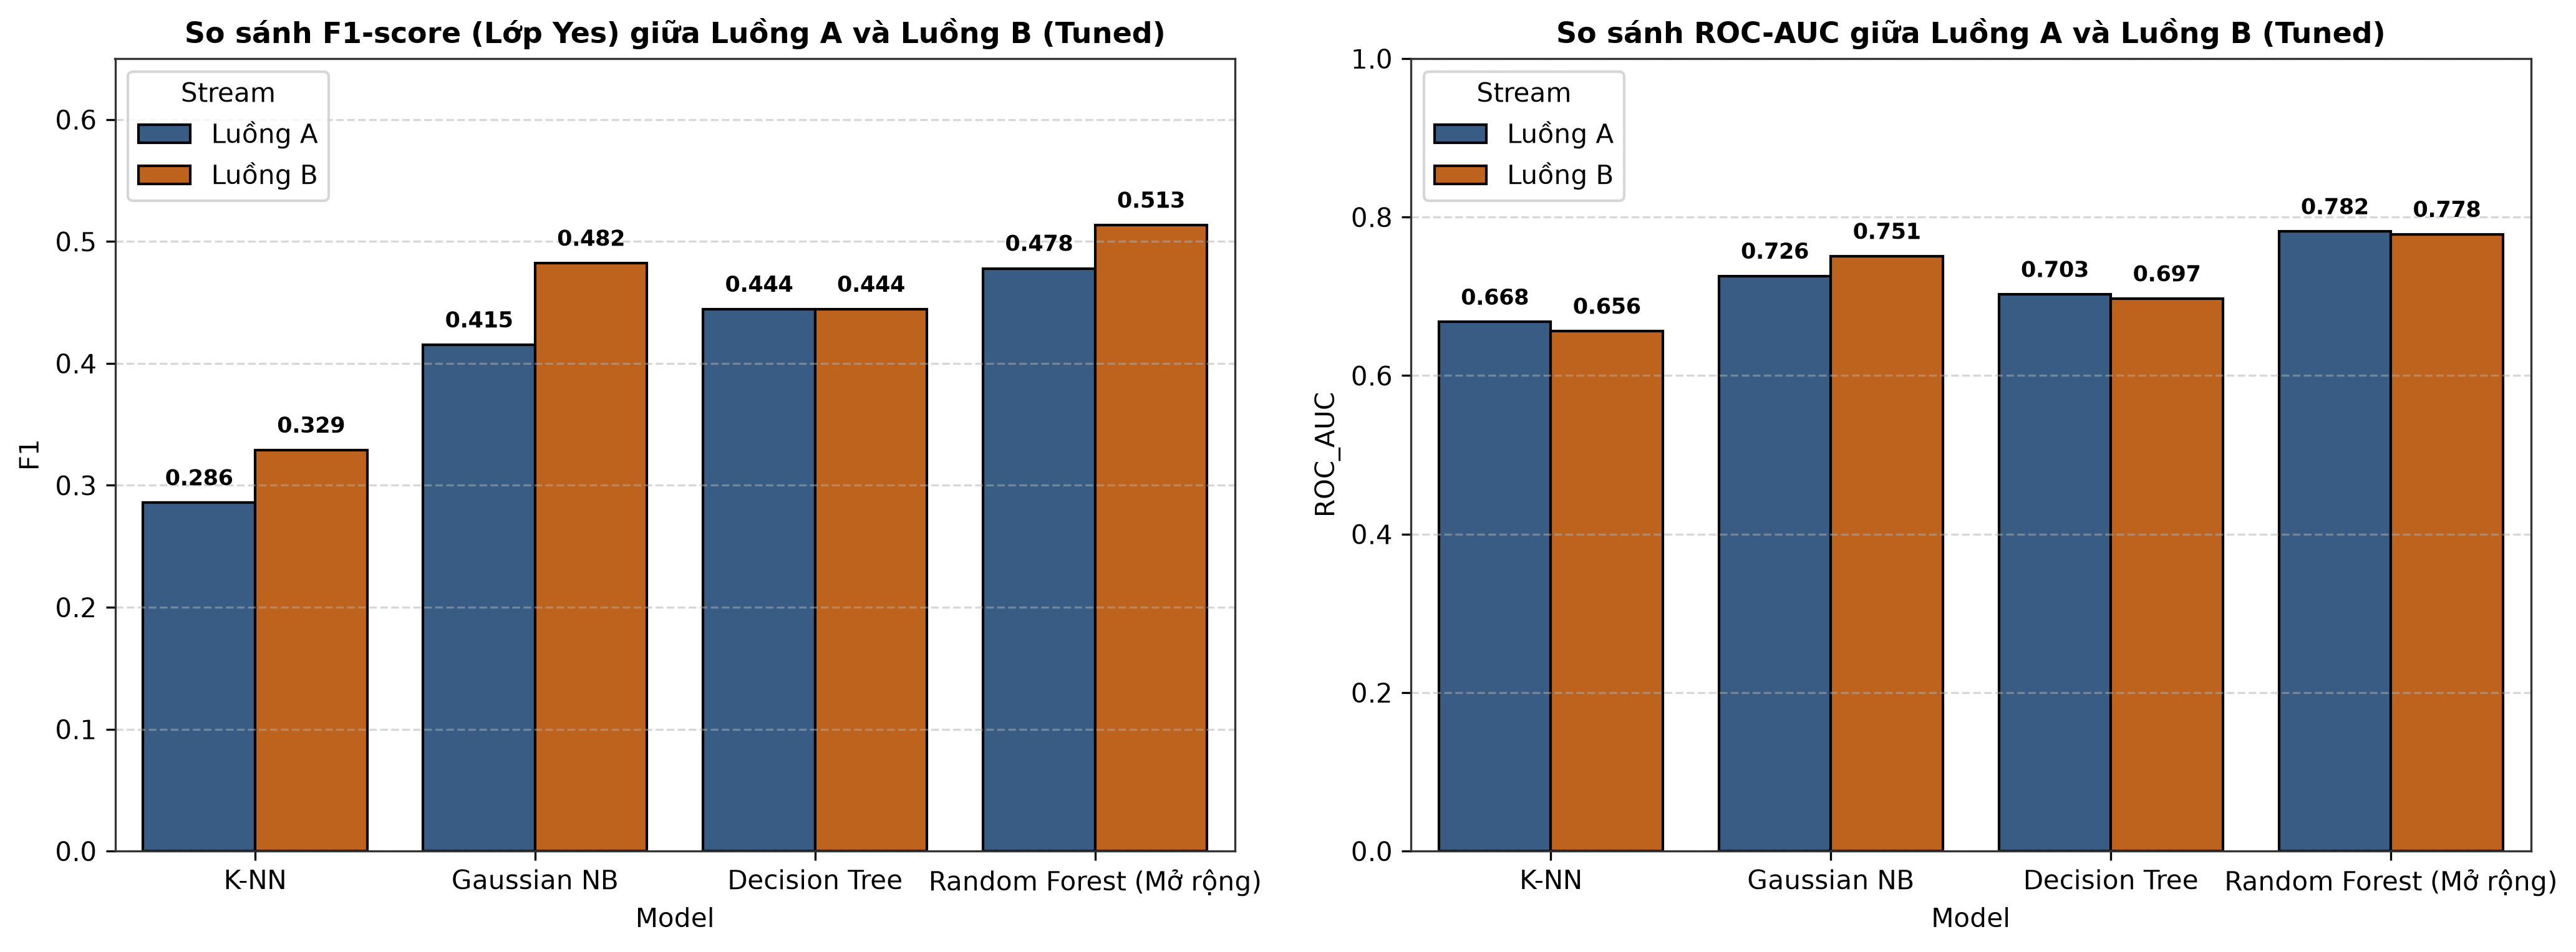
\includegraphics[width=0.98\textwidth]{figures/fig6_model_comparison.png}
    \caption{So sánh F1-score và ROC-AUC giữa Luồng A và Luồng B cho các mô hình đã tinh chỉnh.}
    \label{fig:model_comp}
\end{figure}

\begin{figure}[H]
    \centering
    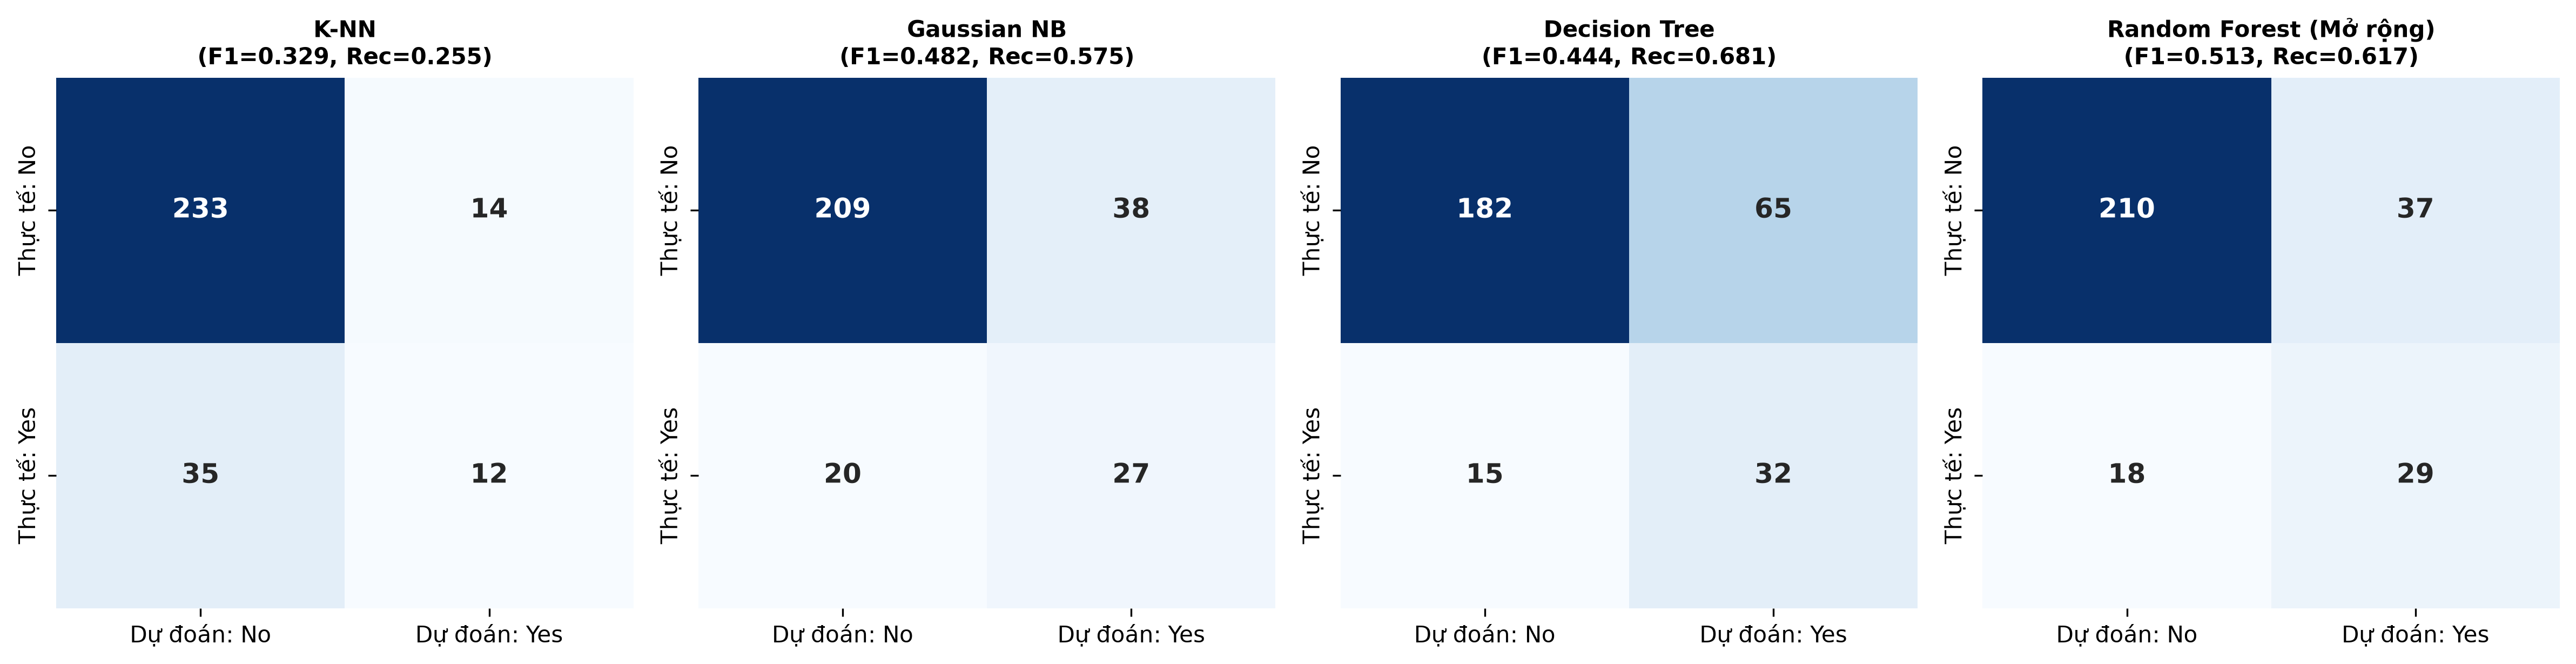
\includegraphics[width=0.99\textwidth]{figures/fig7_confusion_matrices.png}
    \caption{Ma trận nhầm lẫn (Confusion Matrix) của các mô hình đã tinh chỉnh trên Luồng B.}
    \label{fig:cm_plot}
\end{figure}

\begin{figure}[H]
    \centering
    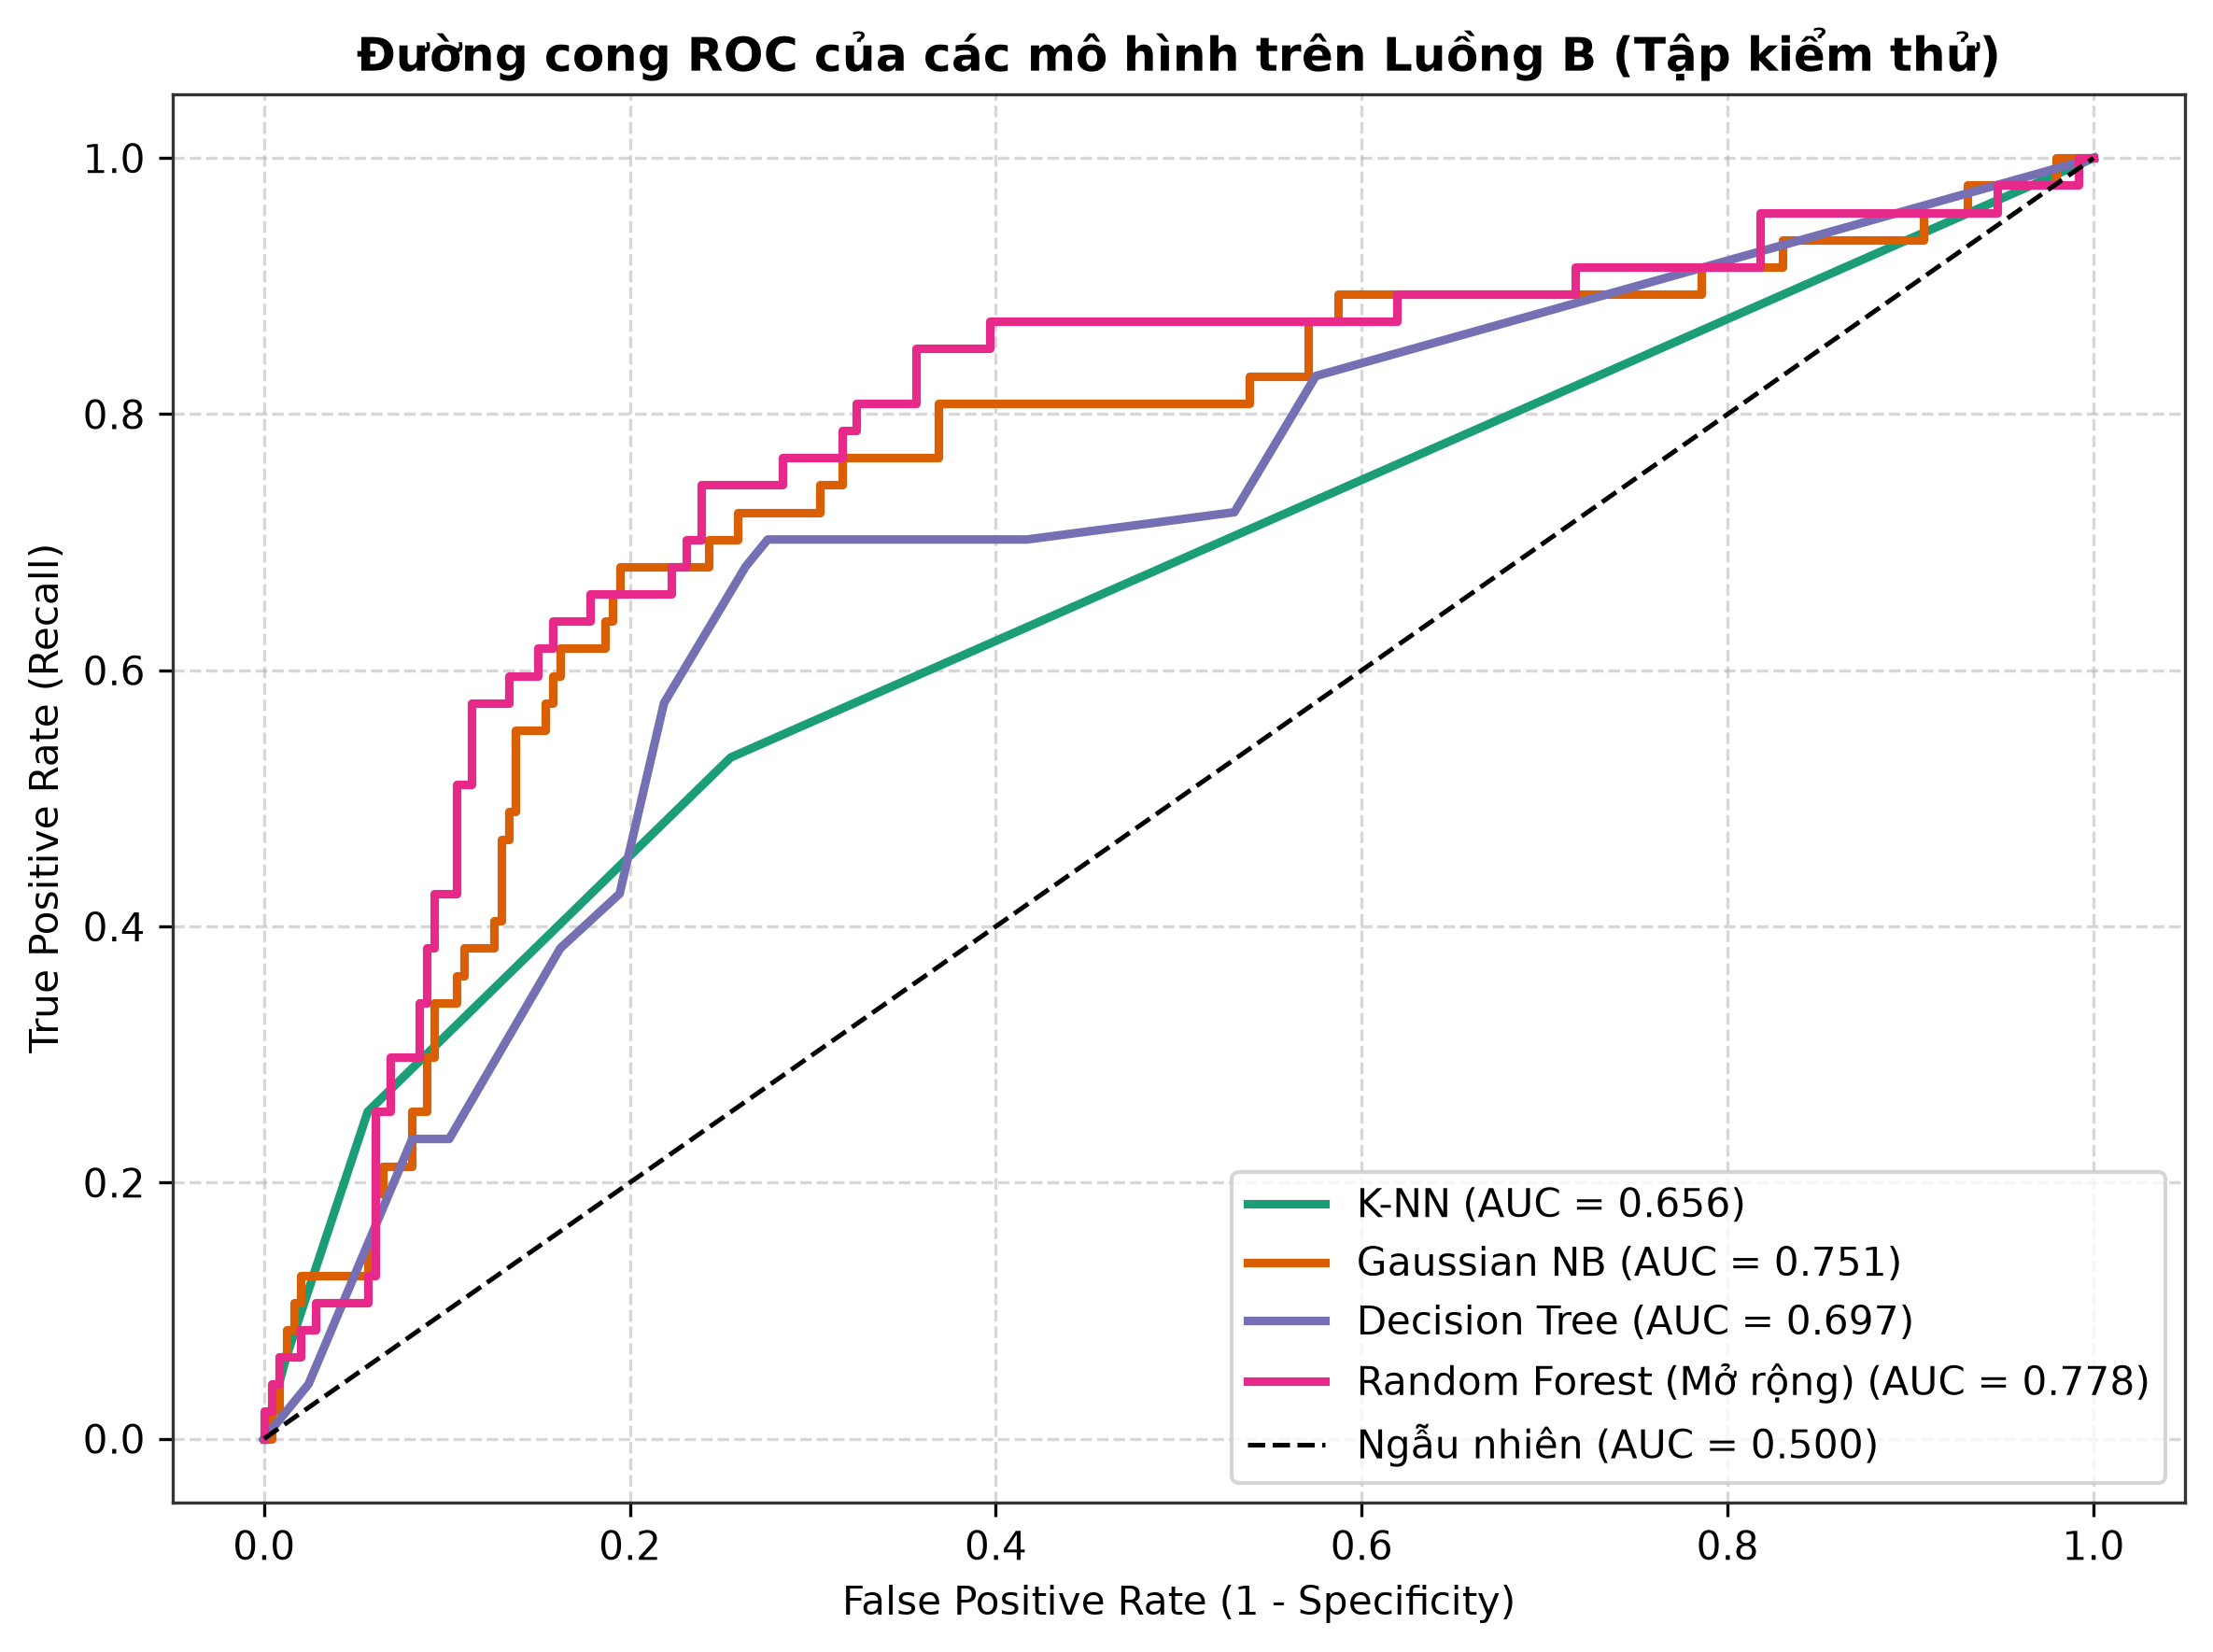
\includegraphics[width=0.72\textwidth]{figures/fig8_roc_curves.png}
    \caption{Đường cong ROC và chỉ số AUC trên tập kiểm thử (Luồng B).}
    \label{fig:roc_plot}
\end{figure}

% =====================================================================
% CHƯƠNG 5: THẢO LUẬN VÀ SO SÁNH
% =====================================================================
\section{Thảo luận và so sánh}

\subsection{Tác động của Luồng B so với Luồng A}
Kết quả trong Bảng \ref{tab:main_results} khẳng định việc cải tiến bước chuẩn bị dữ liệu ở \textbf{Luồng B} mang lại sự cải thiện đồng nhất và có ý nghĩa rõ rệt ở cả trạng thái Mặc định (\texttt{Default}) lẫn Đã tinh chỉnh (\texttt{Tuned}):
\begin{itemize}
    \item \textbf{Ở cấu hình Mặc định (\texttt{Default}):} Chuyển từ Luồng A sang Luồng B giúp \texttt{K-NN} tăng $F_1$ từ $0.1724 \rightarrow 0.2414$ ($+40.0\%$), \texttt{Gaussian NB} tăng $F_1$ từ $0.3687 \rightarrow 0.4526$ ($+22.8\%$) đồng thời giảm số ca báo động giả (\texttt{FP}) từ $99$ xuống $59$ ca, và \texttt{Decision Tree} tăng $F_1$ từ $0.3238 \rightarrow 0.3673$ ($+13.4\%$).
    \item \textbf{Ở cấu hình Đã tinh chỉnh (\texttt{Tuned}):} Trên Luồng B, \texttt{Gaussian NB} đạt $\mathbf{F_1 = 0.4821}$ và $\mathbf{ROC\text{-}AUC = 0.7507}$ (cao nhất trong 3 thuật toán cốt lõi), vượt xa Luồng A ($F_1 = 0.4151$). Tương tự, \texttt{K-NN} tăng $F_1$ từ $0.2857 \rightarrow 0.3288$ và \texttt{Decision Tree} tăng độ nhạy $\text{Recall}$ từ $63.83\% \rightarrow \mathbf{68.09\%}$ (phát hiện được $32/47$ nhân viên nghỉ việc).
    \item \textbf{Nguyên nhân kỹ thuật:} Hình \ref{fig:feat_imp} cho thấy đặc trưng mới \texttt{OverallSatisfaction} và \texttt{CompanyTenureRatio} lọt vào nhóm các biến có độ quan trọng cao nhất của cả Cây quyết định (chiếm $18.73\%$ độ giảm Gini) và Random Forest. Ngoài ra, việc biến đổi $\log(1+x)$ cho các biến lệch phải và loại bỏ biến đa cộng tuyến (\texttt{JobLevel}) giúp thỏa mãn tốt hơn giả định phân phối chuẩn và tính độc lập có điều kiện của \texttt{Gaussian NB}.
\end{itemize}

\begin{figure}[H]
    \centering
    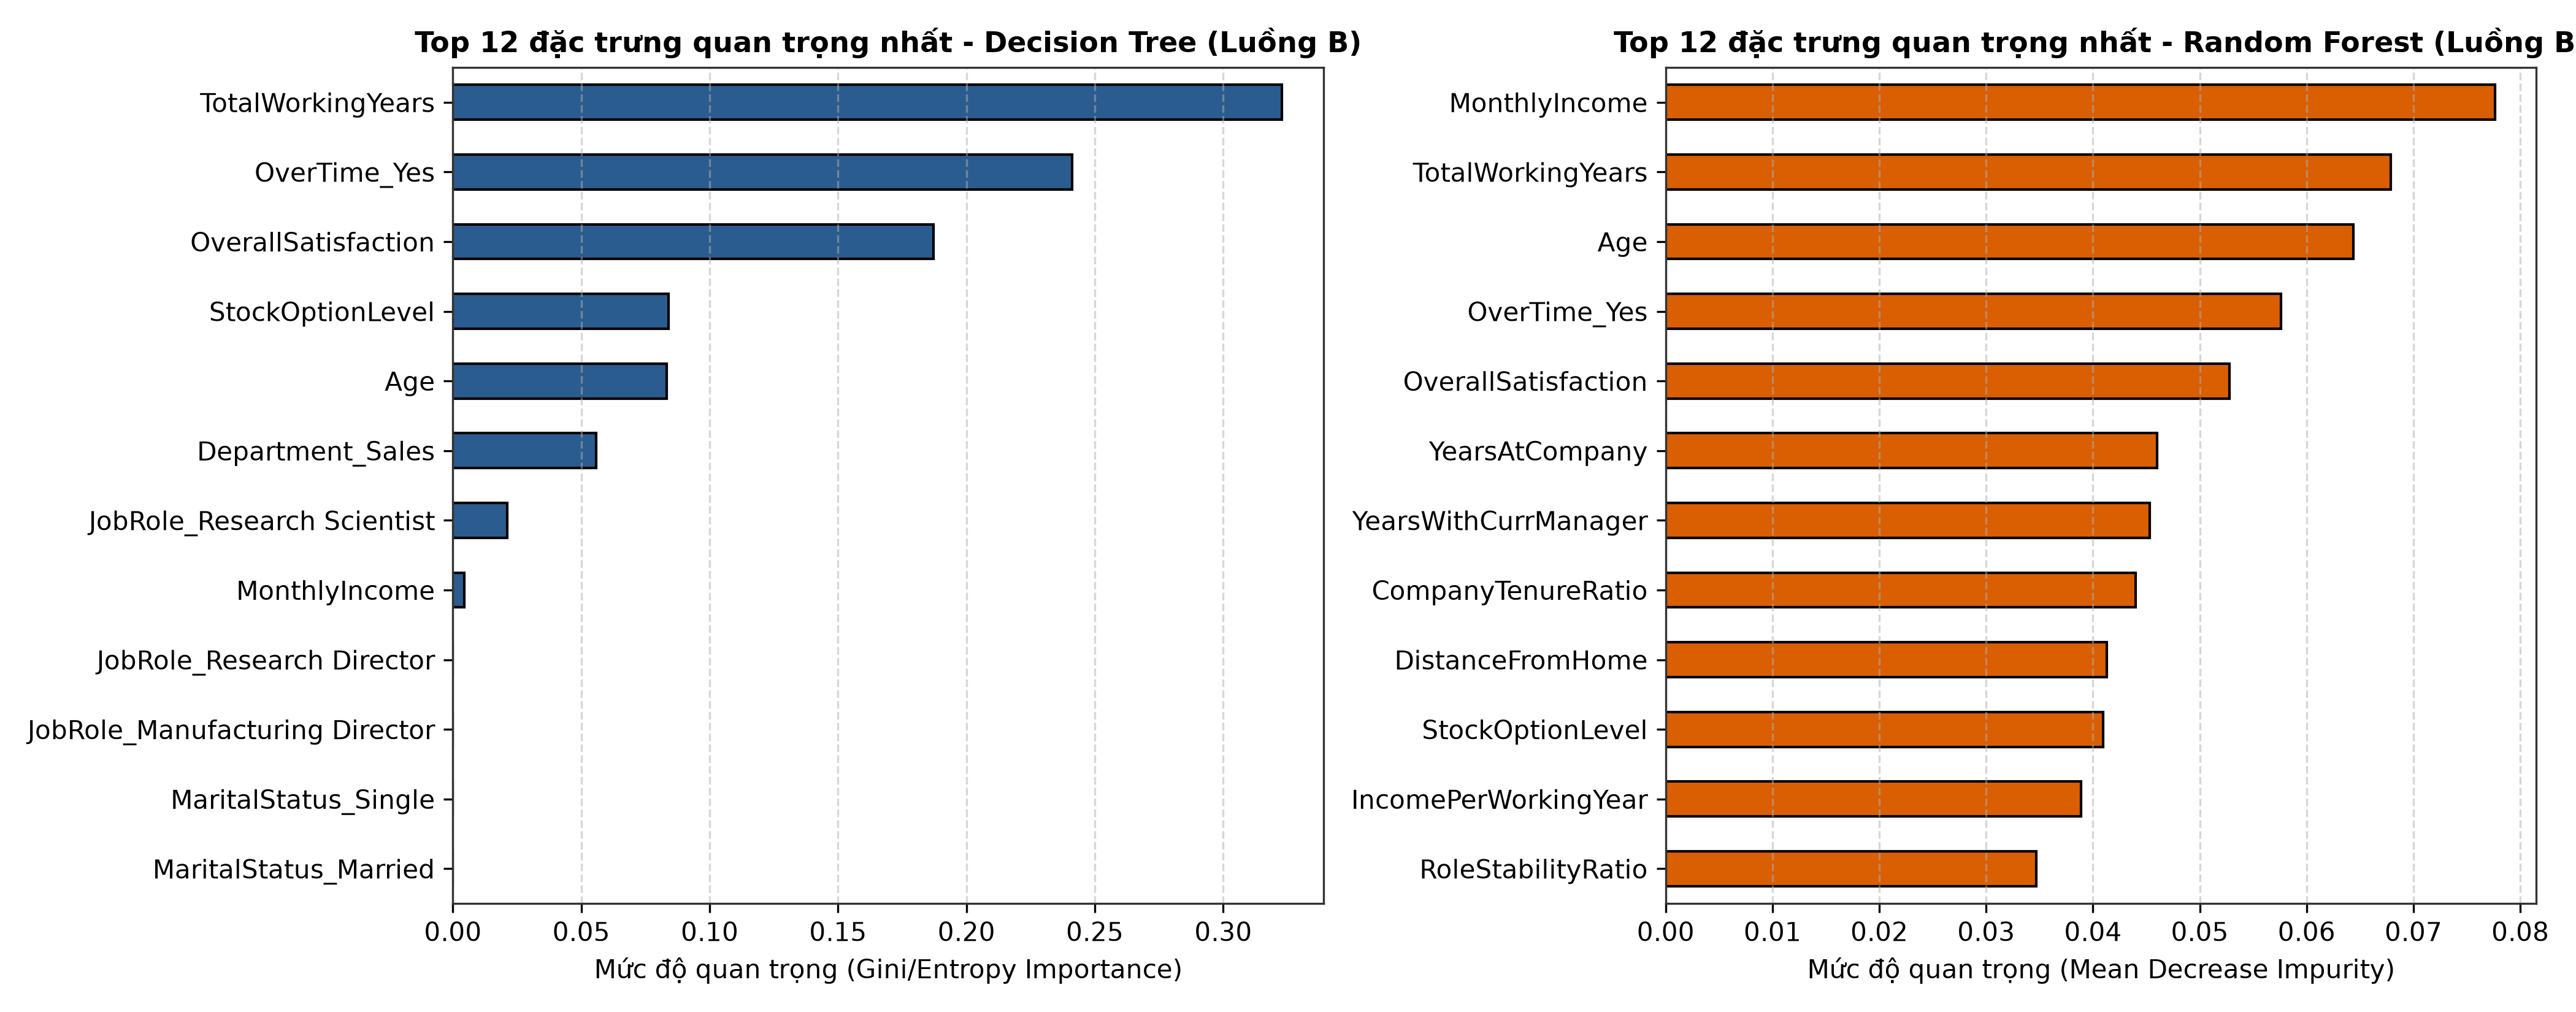
\includegraphics[width=0.98\textwidth]{figures/fig9_feature_importance_tree.png}
    \caption{Top 12 đặc trưng quan trọng nhất trích xuất từ Decision Tree và Random Forest (Luồng B).}
    \label{fig:feat_imp}
\end{figure}

\begin{figure}[H]
    \centering
    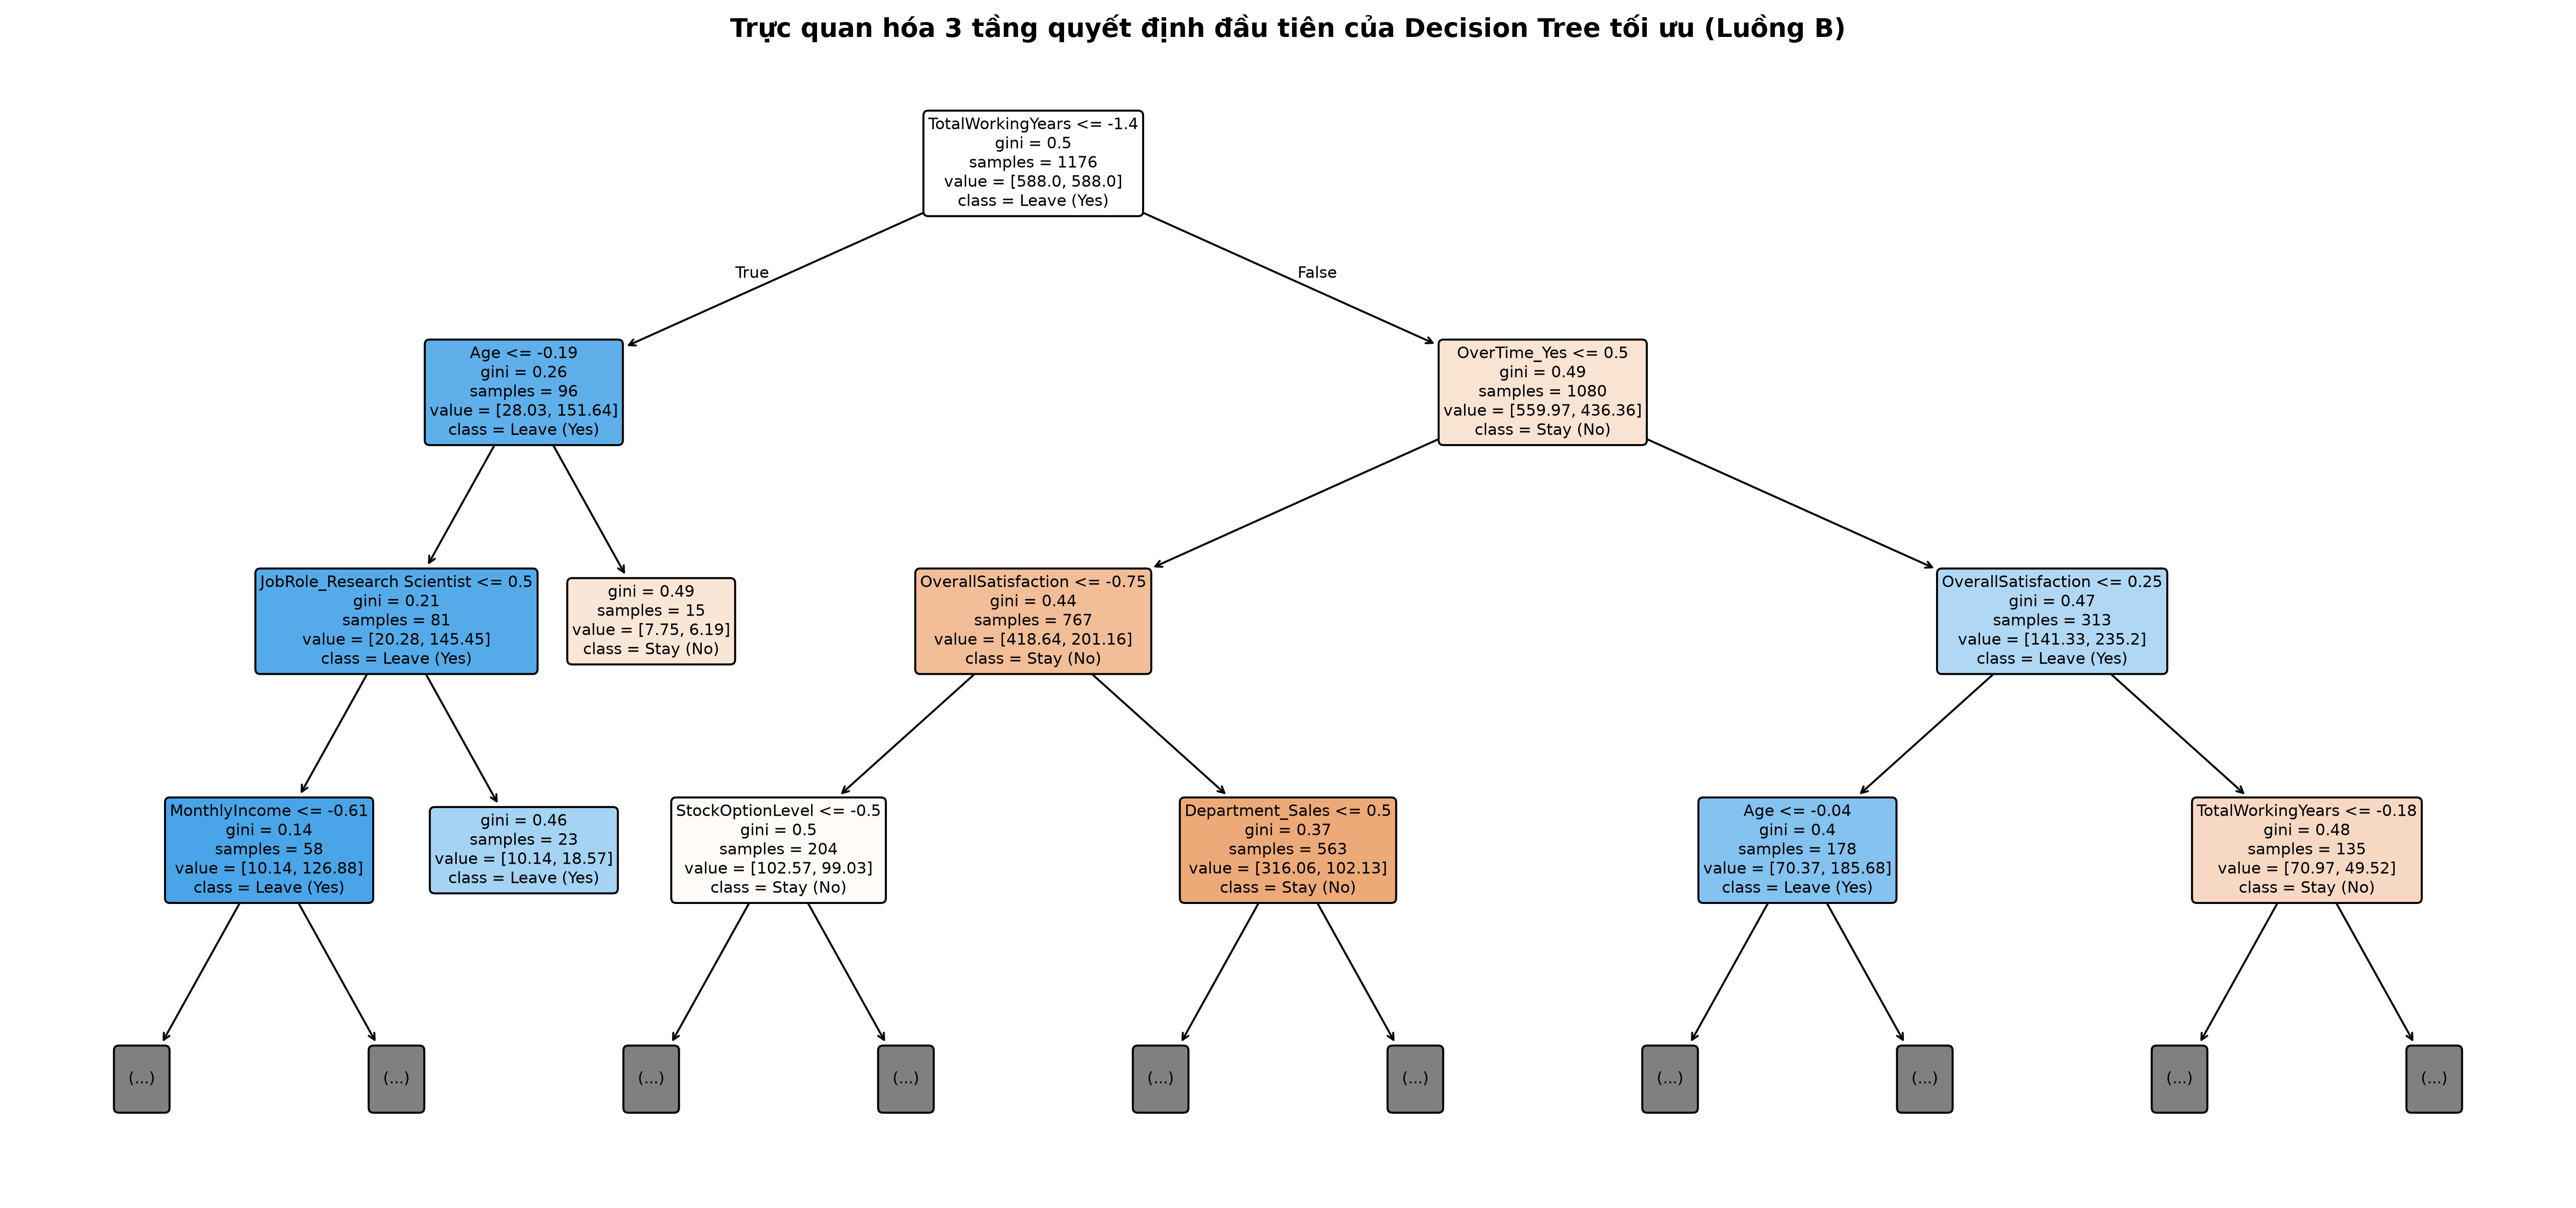
\includegraphics[width=0.99\textwidth]{figures/fig12_decision_tree_structure.png}
    \caption{Trực quan hóa 3 tầng quyết định đầu tiên của mô hình Decision Tree tối ưu trên Luồng B.}
    \label{fig:dt_tree_struct}
\end{figure}

Bên cạnh đó, thực hiện nội dung mở rộng theo Mục 2.4.3 của Hướng dẫn, nhóm khảo sát ảnh hưởng của kỹ thuật giảm chiều bằng Phân tích thành phần chính (\textbf{PCA}) kết hợp với \texttt{K-NN} và \texttt{Gaussian NB}, đồng thời tối ưu hóa ngưỡng xác suất quyết định (\textbf{Decision Threshold Tuning}) cho mô hình \texttt{Random Forest} trên Luồng B (Hình \ref{fig:pca_threshold}). Khi giữ lại $25 - 30$ thành phần chính trực giao, \texttt{PCA + Gaussian NB} loại bỏ hoàn toàn đa cộng tuyến và duy trì $F_1 \approx 0.48$; trong khi tinh chỉnh ngưỡng quyết định về $\tau = 0.525$ giúp \texttt{Random Forest (Luồng B)} đạt đỉnh $\mathbf{F_1 = 0.5192}$ ($\text{Precision} = 47.37\%, \text{Recall} = 57.45\%$).

\begin{figure}[H]
    \centering
    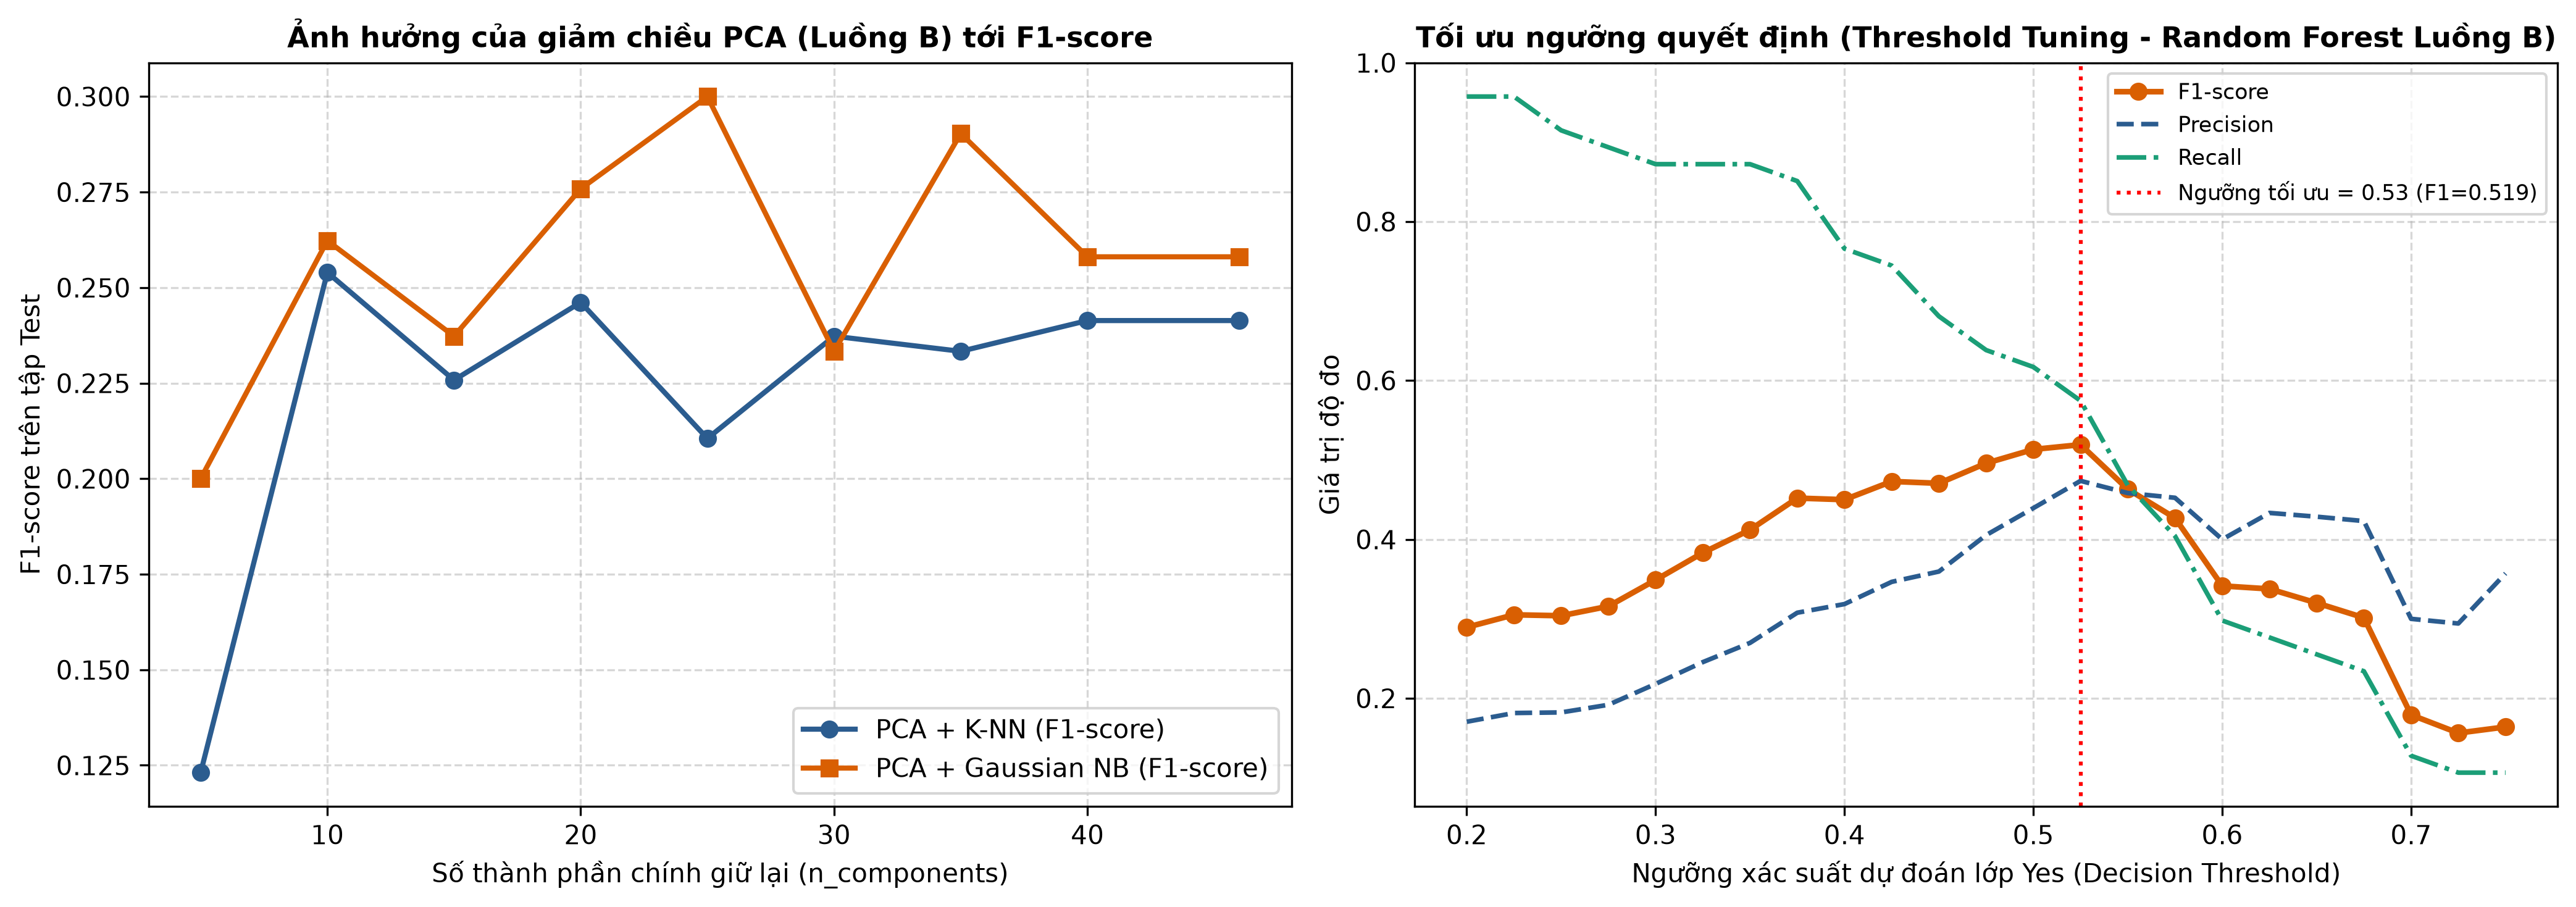
\includegraphics[width=0.98\textwidth]{figures/fig13_pca_and_threshold_tuning.png}
    \caption{Thử nghiệm mở rộng: Giảm chiều bằng PCA và Tinh chỉnh ngưỡng quyết định (Luồng B).}
    \label{fig:pca_threshold}
\end{figure}

\subsection{So sánh ưu, nhược điểm của các thuật toán đã thử nghiệm}
\begin{enumerate}
    \item \textbf{K-Nearest Neighbors (K-NN):}
    \begin{itemize}
        \item \textit{Ưu điểm:} Đạt \texttt{Accuracy} ($83.3\% - 85.0\%$) và \texttt{Precision} khá cao, ít đưa ra cảnh báo giả (\texttt{FP} thấp).
        \item \textit{Nhược điểm:} Độ nhạy \texttt{Recall} thấp nhất ($10.6\% \rightarrow 25.5\%$). Nguyên nhân là do trong không gian nhiều chiều kết hợp dữ liệu mất cân bằng ($83.9\%$ lớp \texttt{No}), láng giềng xung quanh một nhân viên nghỉ việc phần lớn vẫn là các nhân viên ở lại, dẫn đến biểu quyết đa số bị thiên lệch về lớp \texttt{No}.
    \end{itemize}
    \item \textbf{Gaussian Naive Bayes:}
    \begin{itemize}
        \item \textit{Ưu điểm:} Huấn luyện cực nhanh, đạt sự cân bằng tốt nhất giữa \texttt{Precision} ($41.54\%$), \texttt{Recall} ($57.45\%$), $\mathbf{F_1 = 0.4821}$ và $\mathbf{ROC\text{-}AUC = 0.7507}$ khi kết hợp với Luồng B và làm trơn phương sai \texttt{var\_smoothing}.
        \item \textit{Nhược điểm:} Khi dùng trực tiếp trên Luồng A (chưa loại bỏ biến đa cộng tuyến và chưa biến đổi log), mô hình bị phóng đại tỷ số hợp lý (\textit{likelihood ratio}) và sinh ra tới $99$ ca \texttt{False Positives}.
    \end{itemize}
    \item \textbf{Decision Tree (Cây quyết định):}
    \begin{itemize}
        \item \textit{Ưu điểm:} Khả năng diễn giải bạch hộp (\textit{white-box interpretability}) xuất sắc cho bộ phận Nhân sự; khi bật \texttt{class\_weight='balanced'} và cắt tỉa ở \texttt{max\_depth = 4}, mô hình đạt \textbf{Recall cao nhất ($\mathbf{68.09\%}$)}, phát hiện đúng $32/47$ nhân viên nghỉ việc.
        \item \textit{Nhược điểm:} Để đổi lấy \texttt{Recall} cao trên dữ liệu mất cân bằng, cây chấp nhận tỷ lệ \texttt{False Positives} cao hơn ($65$ ca, $\text{Precision} = 32.99\%$). Nếu không giới hạn độ sâu (\texttt{Default}), cây bị quá khớp nặng ($F_1 = 0.3238$).
    \end{itemize}
\end{enumerate}

\subsection{Phân tích lỗi chuyên sâu (Error Analysis)}
Để hiểu rõ tại sao mô hình dự đoán sai, nhóm trích xuất trực tiếp các bản ghi bị phân loại nhầm bởi mô hình \texttt{Decision Tree (Tuned, Luồng B)} trên tập kiểm thử (Bảng \ref{tab:error_cases}).

\begin{table}[H]
\centering
\caption{Các trường hợp dự đoán sai điển hình (\textit{False Negatives} và \textit{False Positives}) trên tập kiểm thử.}
\label{tab:error_cases}
\footnotesize
\begin{tabular}{l c c r c l c c c c}
\toprule
\textbf{Loại lỗi} & \textbf{Mã NV} & \textbf{Tuổi} & \textbf{Lương (\$)} & \textbf{OverTime} & \textbf{Công tác} & \textbf{JobSat} & \textbf{Số năm CT} & \textbf{Năm K.Thăng} & \textbf{Xác suất $\hat{p}$} \\
\midrule
\multirow{4}{*}{\shortstack[l]{\textbf{False Negative}\\(Thực tế: Yes,\\Dự đoán: No)}}
 & \#58   & 41 & 19,545 & No  & Travel\_Rarely     & 3 & 22 & 15 & 0.163 \\
 & \#165  & 58 & 10,312 & No  & Travel\_Rarely     & 4 & 40 & 15 & 0.163 \\
 & \#179  & 51 & 10,650 & No  & Travel\_Frequently & 4 & 4  & 0  & 0.163 \\
 & \#1389 & 31 & 6,179  & Yes & Travel\_Rarely     & 3 & 10 & 6  & 0.252 \\
\midrule
\multirow{4}{*}{\shortstack[l]{\textbf{False Positive}\\(Thực tế: No,\\Dự đoán: Yes)}}
 & \#1495 & 24 & 2,033  & No  & Non-Travel         & 2 & 1  & 0  & 0.958 \\
 & \#1839 & 18 & 1,514  & No  & Non-Travel         & 3 & 0  & 0  & 0.647 \\
 & \#434  & 27 & 2,478  & Yes & Travel\_Rarely     & 2 & 4  & 1  & 0.853 \\
 & \#1297 & 51 & 2,838  & No  & Travel\_Frequently & 3 & 7  & 7  & 0.673 \\
\bottomrule
\end{tabular}
\end{table}

\textbf{Phân tích nguyên nhân và bài học thực tiễn:}
\begin{enumerate}
    \item \textbf{Nhóm lỗi False Negative (FN -- Thực tế nghỉ việc nhưng dự đoán ở lại, gồm 15 ca):}
    Nhìn vào hồ sơ nhân viên \texttt{\#58} (41 tuổi, lương rất cao $\$19{,}545$, không làm thêm giờ, \texttt{JobSatisfaction = 3}) và \texttt{\#165} (58 tuổi, lương $\$10{,}312$, 40 năm làm việc, không làm thêm giờ): bề ngoài đây là những nhân sự cấp cao có chế độ đãi ngộ cực tốt nên mọi mô hình đều gán xác suất nghỉ việc rất thấp ($\hat{p} = 0.163$). Tuy nhiên, cả hai đều có \texttt{YearsSinceLastPromotion = 15 năm} (15 năm không được thăng tiến) hoặc nghỉ hưu sớm / được săn đầu người (\textit{headhunted}). Đây là những trường hợp nghỉ việc do yếu tố ngoại cảnh hoặc bão hòa đỉnh sự nghiệp mà dữ liệu nội bộ hiện tại rất khó tách biệt.
    \item \textbf{Nhóm lỗi False Positive (FP -- Thực tế ở lại nhưng dự đoán nghỉ việc, gồm 65 ca):}
    Các nhân viên như \texttt{\#1495} (24 tuổi, lương thấp $\$2{,}033$, mới vào công ty 1 năm, mức hài lòng thấp $\text{JobSat}=2$) hoặc \texttt{\#434} (27 tuổi, lương $\$2{,}478$, có \texttt{OverTime = Yes}) mang đầy đủ đặc trưng điển hình của nhóm nhân viên hay nghỉ việc. Mặc dù tại thời điểm thu thập dữ liệu họ vẫn đang ở lại (\texttt{Attrition = No}), dưới góc nhìn quản trị nhân sự, các ca \texttt{False Positives} này thực chất là \textbf{nhóm nhân sự có nguy cơ tiềm ẩn cao (\textit{At-risk Employees})} cần được phòng HR quan tâm sớm.
\end{enumerate}

\subsection{Hạn chế của dữ liệu và giải pháp hiện tại}
\begin{itemize}
    \item \textbf{Quy mô mẫu lớp thiểu số nhỏ:} Chỉ có $237$ mẫu lớp \texttt{Yes} trên toàn bộ dữ liệu ($47$ mẫu trên tập kiểm thử), làm giới hạn độ phức tạp tối đa của biên quyết định.
    \item \textbf{Thiếu dữ liệu theo thời gian (\textit{Longitudinal Data}):} Bộ dữ liệu không ghi nhận xu hướng thay đổi mức độ hài lòng hay khối lượng làm thêm giờ qua từng quý trước khi nghỉ việc.
\end{itemize}

% =====================================================================
% CHƯƠNG 6: TỔNG KẾT VÀ HƯỚNG PHÁT TRIỂN
% =====================================================================
\section{Tổng kết và hướng phát triển}

\subsection{Tổng kết kết quả chính và khuyến nghị ứng dụng}
\begin{itemize}
    \item Nhóm đã xây dựng hoàn chỉnh quy trình Học máy từ dữ liệu thô đến đánh giá và phân tích lỗi cho Đề tài 13, đảm bảo tính tái lập cao (\texttt{random\_state = 42}) và ngăn chặn triệt để rò rỉ dữ liệu bằng \texttt{Pipeline}.
    \item Chứng minh thực nghiệm rằng \textbf{Luồng B (Pipeline cải tiến)} với 7 đặc trưng nghiệp vụ HR, biến đổi logarit và chuẩn hóa bền vững (\texttt{RobustScaler}) vượt trội hơn \textbf{Luồng A} trên tất cả các thuật toán cốt lõi.
    \item \textbf{Khuyến nghị triển khai cho phòng Nhân sự (HR):}
    \begin{enumerate}
        \item Sử dụng kết hợp \textbf{Gaussian Naive Bayes (Luồng B)} ($F_1 = 0.4821$, $\text{AUC} = 0.7507$) để xếp hạng xác suất rủi ro và \textbf{Decision Tree (Luồng B)} ($\text{Recall} = 68.09\%$) để trích xuất bộ quy tắc giải thích nguyên nhân.
        \item Tập trung can thiệp vào 3 yếu tố có trọng số quyết định lớn nhất: giảm tải hoặc bù đắp hợp lý cho nhân viên phải làm thêm giờ (\texttt{OverTime = Yes}) kèm công tác thường xuyên; cải thiện chỉ số hài lòng tổng hợp (\texttt{OverallSatisfaction}); và rà soát chế độ lương/cổ phiếu thưởng (\texttt{StockOptionLevel}) cho nhóm nhân viên trẻ độc thân có thâm niên $1 - 3$ năm đầu.
    \end{enumerate}
\end{itemize}

\subsection{Hướng phát triển}
Nếu có thêm thời gian và dữ liệu, dự án có thể được nâng cấp theo các hướng sau:
\begin{enumerate}
    \item Áp dụng kỹ thuật lấy mẫu quá mức tổng hợp (\texttt{SMOTE}) kết hợp hiệu chỉnh ngưỡng xác suất quyết định (\textit{Threshold Tuning}) trên tập Validation để tối ưu hóa hàm chi phí kinh tế giữa chi phí giữ chân (\texttt{FP}) và chi phí mất nhân sự (\texttt{FN}).
    \item Thử nghiệm các mô hình Gradient Boosting hiện đại (\texttt{XGBoost}, \texttt{LightGBM}, \texttt{CatBoost}) kết hợp giải thích mô hình cục bộ bằng giá trị \texttt{SHAP} (\textit{SHapley Additive exPlanations}) cho từng hồ sơ nhân viên.
\end{enumerate}

% =====================================================================
% PHỤ LỤC & TÀI LIỆU THAM KHẢO
% =====================================================================
\appendix
\section{Bảng phân công nhiệm vụ các thành viên Nhóm 7}
Bảng \ref{tab:team_assignment} trình bày chi tiết phân công công việc và mức độ đóng góp của 4 thành viên trong Nhóm 7. Tất cả thành viên đều tham gia thảo luận, rà soát chéo mã nguồn và nắm vững toàn bộ quy trình của nhóm.

\begin{table}[H]
\centering
\caption{Bảng phân công nhiệm vụ và đóng góp của các thành viên Nhóm 7.}
\label{tab:team_assignment}
\footnotesize
\begin{tabular}{c l c p{7.5cm} c}
\toprule
\textbf{STT} & \textbf{Họ và tên} & \textbf{MSSV} & \textbf{Nhiệm vụ phụ trách chính} & \textbf{Tỷ lệ đóng góp} \\
\midrule
1 & Nguyễn Văn An & 1871020003 & Đặt vấn đề, khám phá dữ liệu (EDA), thống kê mô tả, kiểm tra ngoại lệ IQR, phân tích tương quan và biên soạn Chương 1 báo cáo \LaTeX{}. & 25\% \\
\addlinespace
2 & Nguyễn Việt Anh & 1871020047 & Thiết kế kiến trúc Pipeline chống rò rỉ dữ liệu, xây dựng Luồng A và Luồng B (\texttt{HRFeatureEngineer}, \texttt{src/preprocessing.py}), biên soạn Chương 2 \& Chương 3. & 25\% \\
\addlinespace
3 & Đào Thị Tươi & 1871020639 & Huấn luyện mô hình Baseline, tinh chỉnh siêu tham số (\texttt{GridSearchCV}) cho K-NN, Gaussian NB, Decision Tree (\texttt{src/models.py}) và biên soạn Chương 4. & 25\% \\
\addlinespace
4 & Lê Đình Huy & 1871020307 & Đánh giá kết quả, phân tích lỗi (\textit{Error Analysis}), thực nghiệm mở rộng (Random Forest, PCA, Threshold Tuning), xây dựng Demo \texttt{app.py} và biên soạn Chương 5 \& 6. & 25\% \\
\bottomrule
\end{tabular}
\end{table}

\section{Khai báo sử dụng công cụ AI}
Theo quy định tại Mục 2.3 của Hướng dẫn bài tập lớn, nhóm xin khai báo minh bạch việc sử dụng công cụ trợ lý AI trong quá trình thực hiện đề tài:
\begin{itemize}
    \item \textbf{Phạm vi hỗ trợ:} Gợi ý cấu trúc đóng gói \texttt{ColumnTransformer}, \texttt{Pipeline}, lớp \texttt{HRFeatureEngineer} trong thư viện \texttt{scikit-learn}; hỗ trợ tinh chỉnh định dạng đồ thị \texttt{matplotlib/seaborn} và cú pháp bảng biểu/sơ đồ \texttt{TikZ} trong \LaTeX{}.
    \item \textbf{Kiểm chứng và chịu trách nhiệm:} Toàn bộ mã nguồn trong \texttt{DeTai13\_Employee\_Attrition.ipynb} đã được thực thi trên bộ dữ liệu chính thức của Đề tài 13. Mọi con số thống kê, bảng kết quả và ca phân tích lỗi trong báo cáo đều được trích xuất chính xác từ đầu ra thực nghiệm. Các thành viên trong nhóm nắm vững bản chất thuật toán, quy trình xử lý và cam kết giải trình đầy đủ khi bảo vệ.
\end{itemize}

\bibliographystyle{plain}
\bibliography{references}

\end{document}
